\documentclass[12pt,a4paper]{book}
\usepackage[utf8]{inputenc}
\usepackage[T1]{fontenc}
\usepackage[english]{babel}
\usepackage{amsmath}
\usepackage{amsfonts}
\usepackage{amssymb}
\usepackage{geometry}
\geometry{a4paper,left=2.5cm,right=2.5cm,top=2.5cm,bottom=2.5cm}
\usepackage{fancyhdr}
\setlength{\headheight}{30pt}
\usepackage{booktabs}
\usepackage{enumitem}
\usepackage{tcolorbox}
\usepackage{physics}
\usepackage{siunitx}

% Define custom SI units
\DeclareSIUnit\lightyear{ly}
\DeclareSIUnit\gigalightyear{Gly}
\DeclareSIUnit\arcsecond{arcsec}
\DeclareSIUnit\century{century}
\DeclareSIUnit\parsec{pc}
\DeclareSIUnit\megaparsec{Mpc}
\DeclareSIUnit\year{yr}
\DeclareSIUnit\kmpsMpc{km\,s^{-1}\,Mpc^{-1}}
\DeclareSIUnit\mev{MeV}
\DeclareSIUnit\gev{GeV}
\DeclareSIUnit\ev{eV}
\DeclareSIUnit\u{u}

\usepackage{hyperref}
\usepackage{tikz}
\usetikzlibrary{positioning,arrows.meta}

% Hyperref as one of the last packages
\hypersetup{
	unicode=true,
	pdfencoding=unicode,
	bookmarksopen=true,
	pdftitle={Dynamic Vacuum Field Theory (DVFT) - Complete Documentation},
	pdfauthor={},
	pdfsubject={T0-Time-Mass Duality},
	pdfkeywords={DVFT, Fractal Geometry, Quantum Gravity, Cosmology}
}

% Clean PDF bookmarks
\pdfstringdefDisableCommands{%
	\def\Lambda{Lambda}%
	\def\Delta{Delta}%
	\def\approx{approx}%
	\def\Sigma{Sigma}%
	\def\xi{xi}%
	\def\rho{rho}%
	\def\theta{theta}%
	\def\Phi{Phi}%
	\def\cdot{}%
	\def\times{x}%
	\def\hbar{hbar}%
	\def\sqrt#1{sqrt(#1)}%
}

% Header and footer
\pagestyle{fancy}
\fancyhf{}
\fancyhead[LE,RO]{\thepage}
\fancyhead[RE]{\leftmark}
\fancyhead[LO]{\rightmark}

\title{Dynamic Vacuum Field Theory (DVFT)\\
	\large T0-Time-Mass Duality - Complete Documentation}
\author{}
\date{\today}

\begin{document}

\maketitle

\tableofcontents
\newpage

% Chapters 1-11: Foundations
\chapter{Foundations of T0-Time-Mass Duality}
\input{tex_kapitel/202a_1-11_En_section}

% Chapters 12-44: Special Topics
\chapter{Cosmology and the Big-Bang Phase Transition in Fractal T0-Geometry}
In the fractal Fundamental Fractal-Geometric Field Theory (FFGFT), standard expansion cosmology is replaced by a static but dynamically fractal spacetime. What we observe as ``expansion of the universe'' is actually a change in \textbf{fractal depth} and \textbf{scale perception} -- not a physical drifting apart of galaxies in space. The Big Bang was not an explosive beginning, but a phase transition in the fractal vacuum substrate.
	
	\subsection{The Fundamental Illusion: Expansion without Movement}
	
	The apparent redshift of galaxy light \(z\) arises not through Doppler effect, but through fractal scale change:
	
	\textbf{Fractal Redshift:}
	\begin{equation}
		1 + z = \frac{\lambda_{\text{obs}}}{\lambda_{\text{em}}} = \left(\frac{\xi(t_{\text{em}})}{\xi(t_{\text{obs}})}\right)^{-k} = e^{k \cdot \Delta \ln \xi}
	\end{equation}
	
	\textbf{Explanation:}
	\begin{itemize}
		\item \(z\): Redshift (dimensionless)
		\item \(\lambda_{\text{obs}}, \lambda_{\text{em}}\): Observed/emitted wavelength (m)
		\item \(\xi(t)\): Time-dependent fractal scale parameter (dimensionless)
		\item \(k\): Hierarchy level in fractal self-similarity (integer, dimensionless)
		\item \(\Delta \ln \xi = \ln(\xi(t_{\text{obs}})/\xi(t_{\text{em}}))\): Change of the logarithmic scale parameter
	\end{itemize}
	
	The apparent Hubble constant \(H_0\) follows from:
	\begin{equation}
		H_0 = \left|\frac{\dot{\xi}}{\xi}\right|_{t_0} \cdot c \approx 70 \, \text{km/s/Mpc}
	\end{equation}
	with \(\dot{\xi}/\xi \approx -2.27 \times 10^{-18} \, \text{s}^{-1}\).
	
	\subsection{The Big Bang as a Fractal Phase Transition}
	
	The vacuum substrate is described by the fractal field \(\Phi = \rho(x,t) e^{i\theta(x,t)}\), where:
	
	\textbf{Time-Mass Duality manifests as:}
	\begin{equation}
		T(x,t) \cdot m(x,t) = 1
	\end{equation}
	with \(T \propto \theta\) (time structure) and \(m \propto \rho^2\) (mass density).
	
	The Big Bang corresponds to a phase transition:
	
	\textbf{1. Pre-Phase Transition (\(t < t_{\text{BB}}\)):}
	\begin{itemize}
		\item \(\rho \approx 0\): Nearly massless vacuum
		\item \(\theta\): Highly fluctuating, disordered time structure
		\item Fractal depth: Minimal, \(D_f \approx 2\) (strongly underdimensioned)
	\end{itemize}
	
	\textbf{2. Phase Transition (\(t = t_{\text{BB}}\)):}
	\begin{itemize}
		\item Instability: \(\rho\) grows exponentially
		\item \(\theta\) orders itself: Coherent time structure emerges
		\item Fractal dimension stabilizes: \(D_f = 3 - \xi_0\)
	\end{itemize}
	
	\textbf{3. Post-Phase Transition (\(t > t_{\text{BB}}\)):}
	\begin{itemize}
		\item \(\rho = \rho_0 = \frac{\sqrt{\hbar c}}{l_P^{3/2}} \cdot \xi^{-2}\): Stabilized vacuum density
		\item \(\theta\): Uniform time evolution
		\item Fractal depth: \(D_f = 3 - \xi(t)\) with slowly varying \(\xi(t)\)
	\end{itemize}
	
	\subsection{The Fractal Metric without Expansion}
	
	The effective metric describes not expansion, but fractal scale change:
	
	\textbf{Static Fractal Metric:}
	\begin{equation}
		ds^2 = -c^2 dt^2 + \left(\frac{\xi(t_0)}{\xi(t)}\right)^{2/D_f} \left[dr^2 + r^2 d\Omega^2\right]
	\end{equation}
	
	\textbf{Explanation:}
	\begin{itemize}
		\item \(ds^2\): Line element (m\(^2\))
		\item The factor \((\xi(t_0)/\xi(t))^{2/D_f}\): Describes fractal scale change, not expansion
		\item At constant \(\xi\): Reduces to Minkowski metric
		\item At variable \(\xi\): Produces apparent expansion/contraction
	\end{itemize}
	
	The ``scale function'' \(a(t)\) of standard cosmology is replaced by:
	
	\begin{equation}
		a_{\text{eff}}(t) = \left(\frac{\xi(t_0)}{\xi(t)}\right)^{1/D_f}
	\end{equation}
	
	This quantity describes not a physical expansion, but the fractal scale perception.
	
	\subsection{Evolution of the Fractal Parameter \(\xi(t)\)}
	
	The time dependence of \(\xi\) follows from vacuum stability:
	
	\textbf{Differential Equation:}
	\begin{equation}
		\frac{d\xi}{dt} = -\frac{\xi^2}{\tau_0} \cdot \left(1 - \frac{\xi}{\xi_{\infty}}\right)
	\end{equation}
	
	\textbf{Solution:}
	\begin{equation}
		\xi(t) = \frac{\xi_0 \xi_{\infty} e^{-t/\tau_0}}{\xi_{\infty} - \xi_0 + \xi_0 e^{-t/\tau_0}}
	\end{equation}
	
	\textbf{Parameters:}
	\begin{itemize}
		\item \(\xi_0 = \frac{4}{3} \times 10^{-4}\): Initial value at \(t_{\text{BB}}\)
		\item \(\xi_{\infty} \approx 1.2 \times 10^{-4}\): Final value for \(t \to \infty\)
		\item \(\tau_0 = \frac{\hbar}{m_P c^2 \xi_0^2} \approx 4.3 \times 10^{17} \, \text{s}\): Characteristic time
	\end{itemize}
	
	\subsection{Cosmic Microwave Background Radiation (CMB)}
	
	The CMB arises not from a hot primordial phase, but from fractal vacuum fluctuations:
	
	\textbf{Temperature Distribution:}
	\begin{equation}
		T_{\text{CMB}}(\theta, \phi) = T_0 \left[1 + \sum_{l,m} a_{lm} Y_{lm}(\theta, \phi)\right]
	\end{equation}
	
	\textbf{with:}
	\begin{equation}
		a_{lm} \propto \int \frac{\delta \rho(\vec{x})}{\rho_0} \cdot j_l(kr) \cdot Y_{lm}^*(\theta, \phi) d^3x
	\end{equation}
	
	\textbf{Fractal Density Fluctuations:}
	\begin{equation}
		\frac{\delta \rho(\vec{x})}{\rho_0} = \xi \cdot \sum_n \frac{\cos(2\pi |\vec{x} - \vec{x}_n|/\lambda_n)}{|\vec{x} - \vec{x}_n|^{D_f/2}}
	\end{equation}
	
	The characteristic anisotropies (\(l \approx 220\) maximum) arise from fractal resonance at scales:
	\begin{equation}
		\lambda_{\text{res}} = \frac{2\pi c}{H_0} \cdot \frac{D_f}{2} \approx 1.1 \times 10^{26} \, \text{m}
	\end{equation}
	
	\subsection{Baryon Acoustic Oscillations (BAO)}
	
	The BAO scale arises through fractal standing waves in the early vacuum:
	
	\textbf{Characteristic Scale:}
	\begin{equation}
		r_{\text{BAO}} = \frac{\pi c}{H_0} \cdot \frac{1}{\sqrt{1 - \xi/2}} \approx 150 \, \text{Mpc}
	\end{equation}
	
	This scale appears in the galaxy correlation function as a peak at:
	\begin{equation}
		\xi_{\text{gal}}(r) \propto \frac{\sin(r/r_{\text{BAO}})}{r/r_{\text{BAO}}} \cdot r^{-(3-D_f)}
	\end{equation}
	
	\subsection{Dark Energy as Fractal Scale Change}
	
	What is interpreted as Dark Energy is the continued fractal evolution:
	
	\textbf{Effective Dark Energy Density:}
	\begin{equation}
		\rho_{\Lambda}^{\text{eff}} = \frac{3H_0^2}{8\pi G} \cdot \left(\frac{\dot{\xi}}{\xi H_0}\right)^2 \approx 0.7 \rho_c
	\end{equation}
	
	\textbf{Equation of State:}
	\begin{equation}
		w_{\text{eff}} = -1 + \frac{2}{3} \cdot \frac{\ddot{\xi}\xi}{\dot{\xi}^2} \approx -0.98
	\end{equation}
	
	These values agree with observations (\(\Omega_\Lambda \approx 0.7\), \(w \approx -1\)), but require no mysterious energy form.
	
	\subsection{Structure Formation without Inflation}
	
	The apparent homogeneity and flatness arise naturally from fractal self-similarity:
	
	\textbf{Horizon Problem:} Solved by fractal non-locality -- all points are connected on small scales
	
	\textbf{Flatness Problem:} The fractal metric is intrinsically flat (\(k=0\)) on all scales
	
	\textbf{Monopole Problem:} Fractal topology allows no topological defects with dangerous density
	
	\subsection{Testable Predictions}
	
	\textbf{1. Deviations from Standard-\(\Lambda\)CDM:}
	\begin{equation}
		\frac{\Delta C_l}{C_l^{\Lambda\text{CDM}}} = \xi \cdot \ln\left(\frac{l}{l_0}\right) \quad \text{for } l > 100
	\end{equation}
	At \(l = 2000\): \(\Delta C_l/C_l \approx 0.1\%\)
	
	\textbf{2. Time Variation of Fundamental Constants:}
	\begin{equation}
		\frac{\dot{\alpha}}{\alpha} = -2 \frac{\dot{\xi}}{\xi} \approx 4.5 \times 10^{-18} \, \text{s}^{-1}
	\end{equation}
	Testable with atomic clocks and quasar absorption.
	
	\textbf{3. Fractal Correlations in LSS:}
	\begin{equation}
		P(k) = P_{\Lambda\text{CDM}}(k) \cdot \left[1 + \xi \cdot (k/k_0)^{-D_f+3}\right]
	\end{equation}
	For \(k_0 = 0.1 \, \text{h/Mpc}\): Deviations at small \(k\).
	
	\subsection{Comparison with Standard-\(\Lambda\)CDM}
	
	\begingroup
	\small
	\begin{tabular}{p{0.45\textwidth}|p{0.45\textwidth}}
		\textbf{Standard-\(\Lambda\)CDM} & \textbf{Fractal T0-Cosmology} \\
		\hline
		Space expands physically & Space is static, fractal depth changes \\
		Big Bang: Singularity & Big Bang: regular phase transition with tiny but finite core scale $L_0 \sim 1/\xi$ \\
		Dark Matter: Particles & Dark Matter: Fractal geometry \\
		Dark Energy: Constant \(\Lambda\) & Dark Energy: Fractal scale evolution \\
		Inflation needed for homogeneity & Fractal self-similarity guarantees homogeneity \\
		6+ free parameters & 1 parameter: \(\xi_0 = \frac{4}{3} \times 10^{-4}\) \\
		Horizons through causal delay & Fractal non-locality connects all points \\
		Redshift: Doppler effect & Redshift: Fractal scale change \\
	\end{tabular}
	\endgroup
	
	\subsection{Temporal Evolution in T0}
	
	\begin{enumerate}
		\item \textbf{Early fractal era} (\(t < 10^{-32}\) s): \(\xi \approx \xi_0\), \(D_f \approx 3 - \xi_0\)
		\item \textbf{Radiation-like phase} (\(10^{-32}\) s \(< t < 4.7 \times 10^4\) years): \(\xi\) slowly decreasing
		\item \textbf{Matter-like phase} (\(4.7 \times 10^4\) years \(< t < 9.8 \times 10^9\) years): \(\dot{\xi}/\xi\) approximately constant
		\item \textbf{Scale-change dominated} (\(t > 9.8 \times 10^9\) years): \(\dot{\xi}/\xi\) dominates energy balance
	\end{enumerate}
	
	\subsection{The Universe as a Deepening Brain: A Narrative Synthesis}
	
	The formal mathematical description of T0-cosmology finds its most complete and intuitive analogy in the image of a developing brain. This poetic, yet scientifically founded image summarizes the essence of the theory:
	
	\begin{center}
		\begin{tikzpicture}[
			node distance=1cm and 2cm,
			box/.style={rectangle, draw=black!50, thick, minimum width=3cm, minimum height=1.2cm, align=center, rounded corners=3pt, text width=2.8cm},
			arrow/.style={->, >=stealth, thick},
			scale=0.85,
			transform shape
			]
			
			% Nodes
			\node (grund) [box, fill=blue!10] {Ground State \\ ``Flat'' fractal vacuum \\ $D_f \approx 2$, high $\xi$};
			\node (phase) [box, fill=orange!10, below=of grund] {Big Bang as \\ Phase Transition};
			\node (entwicklung) [box, fill=green!10, below=of phase] {Evolution \\ \& ``Deepening''};
			
			% Lower row
			\node (exp) [box, fill=red!10, below left=1cm and -1.5cm of entwicklung] {``Expansion'' \\ \& Redshift \\ Scale perception \\ shifts};
			\node (struktur) [box, fill=purple!10, below=1cm of entwicklung] {Structure Formation \\ CMB patterns, \\ Galaxies};
			\node (energie) [box, fill=teal!10, below right=1cm and -1.5cm of entwicklung] {``Dark Energy'' \\ Residual effect \\ of deepening};
			
			% Observations
			\node (hubble) [box, fill=red!5, below=0.7cm of exp] {Observation: \\ $H_0 \approx 70$ km/s/Mpc};
			\node (cmb) [box, fill=purple!5, below=0.7cm of struktur] {Observation: \\ CMB anisotropies, \\ BAO scale};
			\node (beschl) [box, fill=teal!5, below=0.7cm of energie] {Observation: \\ Accelerated \\ ``Expansion'' \\ ($\Omega_\Lambda \approx 0.7$)};
			
			% Conclusion Box
			\node (fazit) [box, fill=yellow!20, below=1.2cm of cmb, minimum width=8cm, text width=7.5cm] {Conclusion: Static, deepening ``brain-universe'' \\ replaces expanding balloon model};
			
			% Arrows
			\draw [arrow] (grund) -- (phase);
			\draw [arrow] (phase) -- (entwicklung);
			\draw [arrow] (entwicklung) -- (exp);
			\draw [arrow] (entwicklung) -- (struktur);
			\draw [arrow] (entwicklung) -- (energie);
			\draw [arrow] (exp) -- (hubble);
			\draw [arrow] (struktur) -- (cmb);
			\draw [arrow] (energie) -- (beschl);
			
			% Arrows to conclusion
			\draw [arrow] (hubble.south) to[out=-90, in=180] ([xshift=-10pt]fazit.west);
			\draw [arrow] (cmb) -- (fazit);
			\draw [arrow] (beschl.south) to[out=-90, in=0] ([xshift=10pt]fazit.east);
			
		\end{tikzpicture}
	\end{center}
	
	\textbf{The brain analogy deepens in several dimensions:}
	
	\begin{itemize}
		\item \textbf{Convolutions instead of Expansion}: A developing brain doesn't simply grow as a whole, but forms complex folds and convolutions that dramatically increase its surface area at constant volume. The T0-universe doesn't ``expand'' -- it \textit{deepens}. The fractal dimension $D_f = 3 - \xi(t)$ describes precisely this increasing complexity and ``surface area'' of spacetime.
		
		\item \textbf{Neural Network \& Cosmic Web}: The large-scale structure of the universe with its galaxy filaments and voids is not a random product of gravitation, but a standing fractal pattern that bears a striking resemblance to neural connections in the brain. The equation $\delta\rho/\rho_0 = \xi \cdot \sum_n \cos(2\pi|\vec{x}-\vec{x}_n|/\lambda_n) / |\vec{x}-\vec{x}_n|^{D_f/2}$ describes these ``cosmic neurons'' as resonances in the vacuum substrate.
		
		\item \textbf{Information Processing}: A brain processes sensory impressions into thoughts. The T0-vacuum ``processes'' via the Time-Mass Duality $T(x,t) \cdot m(x,t) = 1$ pure time structure ($\theta$) into manifest mass/energy ($\rho$) and back. The Big-Bang phase transition was the moment when the ``universal brain'' began to ``think'' -- from a disordered phase fluctuation to a coherent, structured reality.
		
		\item \textbf{Self-Similarity}: Like a brain organized self-similarly at different scales (from synapses through neuron groups to entire brain areas), the T0-universe is self-similar through the fractal dimension $D_f$ at all scales -- from the Planck length to the cosmic horizon.
		
		\item \textbf{Horizon Problem as Global Networking}: A brain despite its size has no ``horizon problems'' -- information is globally available through networking. The fractal non-locality of the T0-vacuum provides instantaneous correlations at all scales, which explains the astonishing homogeneity of the CMB.
		
		\item \textbf{Dark Energy as Metabolism}: The observed ``accelerated expansion'' (Dark Energy) is not a mysterious drive, but the energetic basal metabolic rate of the deepening system -- the residual effect $\rho_\Lambda^{\text{eff}} = (3H_0^2/8\pi G) \cdot (\dot{\xi}/\xi H_0)^2$, analogous to the metabolism of an active brain.
	\end{itemize}
	
	\subsection{Conclusion: A New Paradigm of Reality}
	
	Fractal T0-cosmology revolutionizes our understanding of the universe through a radical reinterpretation:
	
	\begin{center}
		\textbf{We do not live in an expanding balloon,} \\
		\textbf{but in a deepening, folding, self-similar fabric --} \\
		\textbf{a cosmic brain, whose ``convolutions'' continuously become} \\
		\textbf{more pronounced through the fractal Time-Mass Duality.}
	\end{center}
	
	The observed ``expansion'' is merely our perspective effect, as we ``zoom'' into this increasing fractal depth. This view eliminates singularities, Dark Energy as a separate entity, and reduces all cosmology to a single, elegant geometric principle: the dynamic self-organization of a fractal vacuum.
	
	The T0-theory thus shows that a static, deepening universe with dynamic geometry can explain all observations of modern cosmology -- without actual expansion, without additional components like Dark Matter, and with only one fundamental parameter: $\xi_0 = \frac{4}{3} \times 10^{-4}$.


\chapter{Chronology of Universe Creation from Fractal Time-Mass Duality}
\input{tex_kapitel/kapitel_13a_En_section}

\chapter{Space Creation as Fractal Amplitude Front in T0-Time-Mass Duality}
In T0-Time-Mass Duality, physical space exists only where the fractal vacuum amplitude $\rho(\vec{x},t) > 0$ is. The apparent ''expansion'' of the universe is actually the propagation of an amplitude front that ''creates'' physical space by transitioning the fractal vacuum from a pre-state ($\rho \approx 0$) to a stable state ($\rho = \rho_0$). This process is completely determined by the parameter $\xi = \frac{4}{3} \times 10^{-4}$ and is a direct consequence of the Time-Mass Duality.
	
	\subsection{Symbol Directory and Units}
	
	\begin{tcolorbox}[title={\textbf{Important Symbols and their Units}}, colback=blue!5!white, colframe=blue!75!black]
		\begin{tabular}{p{0.3\textwidth}p{0.3\textwidth}p{0.35\textwidth}}
			\textbf{Symbol} & \textbf{Meaning} & \textbf{Unit (SI)} \\
			\hline
			$\xi$ & Fractal scale parameter & dimensionless \\
			$\rho(\vec{x},t)$ & Vacuum amplitude density & $\si{\kilo\gram^{1/2}\per\meter^{3/2}}$ \\
			$\rho_0$ & Vacuum equilibrium density & $\si{\kilo\gram^{1/2}\per\meter^{3/2}}$ \\
			$T(x,t)$ & Time density & $\si{\second\per\meter^{3}}$ \\
			$m(x,t)$ & Mass density & $\si{\kilo\gram\per\meter^{3}}$ \\
			$v_b(t)$ & Front velocity & $\si{\meter\per\second}$ \\
			$c$ & Speed of light & $\SI{2.9979e8}{\meter\per\second}$ \\
			$R(t)$ & Front position & $\si{\meter}$ \\
			$l_0$ & Fractal correlation length & $\si{\meter}$ \\
			$l_P$ & Planck length & $\SI{1.616e-35}{\meter}$ \\
			$t_0$ & Present age of universe & $\SI{4.35e17}{\second}$ \\
			$H_0$ & Hubble constant & $\SI{2.27e-18}{\per\second}$ \\
			$D_f$ & Fractal dimension & dimensionless \\
		\end{tabular}
	\end{tcolorbox}
	
	\subsection{The Fundamental Principle: Space Emerges from Amplitude}
	
	\textbf{Time-Mass Duality as Motor of Space Creation:}
	\begin{equation}
		\tilde{T}(x,t) \cdot \tilde{m}(x,t) = 1 \quad \text{with} \quad \tilde{T} = T \cdot l_P^3, \quad \tilde{m} = m \cdot \frac{l_P^3}{m_P}
	\end{equation}
	
	\textbf{Unit Check:}
	\begin{align*}
		[\tilde{T}] &= [T] \cdot [l_P^3] = \si{\second\per\meter^{3}} \cdot \si{\meter^{3}} = \si{\second} \\
		[\tilde{m}] &= [m] \cdot \frac{[l_P^3]}{[m_P]} = \si{\kilo\gram\per\meter^{3}} \cdot \frac{\si{\meter^{3}}}{\si{\kilo\gram}} = \text{dimensionless} \\
		[\tilde{T} \cdot \tilde{m}] &= \si{\second} \cdot \text{dimensionless} = \si{\second} \quad \text{(dimensionless product correct)}
	\end{align*}
	
	\textbf{Explanation of Duality:}
	\begin{itemize}
		\item For $\rho = 0$: $m \approx 0$, therefore $\tilde{m} \approx 0$ and $\tilde{T} \to \infty$ (unstable state)
		\item For $\rho = \rho_0$: $m = \rho_0^2$, therefore $\tilde{m} = \text{constant}$ and $\tilde{T} = 1/\tilde{m}$ (stable state)
		\item The transition $\rho: 0 \to \rho_0$ ''creates'' physical space
		\item The front velocity $v_b(t)$ determines the ''expansion rate''
	\end{itemize}
	
	\subsection{Fundamental Amplitude Equation with Fractal Corrections}
	
	From the fractal action with Time-Mass Duality results the effective Lagrange density:
	
	\begin{equation}
		\mathcal{L}[\rho] = \frac{1}{2}(\partial_t\rho)^2 - \frac{c^2}{2}(\nabla\rho)^2 - V(\rho) + \xi \cdot \mathcal{L}_{\text{frac}}[\rho]
	\end{equation}
	
	\textbf{Unit Check:}
	\begin{align*}
		[\mathcal{L}] &= \si{\joule\per\meter^{3}} = \si{\kilo\gram\per\meter\second^{2}} \\
		[(\partial_t\rho)^2] &= \left(\frac{\si{\kilo\gram^{1/2}\per\meter^{3/2}}}{\si{\second}}\right)^2 = \si{\kilo\gram\per\meter^{3}\second^{2}} \\
		[c^2(\nabla\rho)^2] &= \si{\meter^{2}\per\second^{2}} \cdot \left(\frac{\si{\kilo\gram^{1/2}\per\meter^{3/2}}}{\si{\meter}}\right)^2 = \si{\kilo\gram\per\meter^{3}\second^{2}} \\
		\text{Units consistent}
	\end{align*}
	
	\textbf{The Correct Potential:}
	\begin{equation}
		V(\rho) = \frac{\lambda}{4} m_P^2 c^4 \left(\frac{\rho^2}{\rho_P^2} - 1\right)^2
	\end{equation}
	\begin{align*}
		[m_P^2 c^4] &= \si{\kilo\gram^{2}} \cdot \si{\meter^{8}\per\second^{4}} = \si{\kilo\gram^{2}\meter^{8}\per\second^{4}} \\
		\left[\frac{\rho^2}{\rho_P^2}\right] &= \text{dimensionless} \\
		[V] &= [\lambda] \cdot \si{\kilo\gram^{2}\meter^{8}\per\second^{4}} \\
		\text{For } [V] = \si{\kilo\gram\per\meter\second^{2}} \text{ must have } [\lambda] = \si{\per\kilo\gram\meter^{9}\second^{2}}
	\end{align*}
	
	\textbf{Fractal Correction Terms:}
	\begin{equation}
		\mathcal{L}_{\text{frac}}[\rho] = \sum_{n=1}^\infty \xi^{n-1} \cdot l_0^{2n-2} \cdot (\nabla^n\rho)^2
	\end{equation}
	\begin{align*}
		[\nabla^n\rho] &= \si{\kilo\gram^{1/2}\per\meter^{3/2+n}} \\
		[(\nabla^n\rho)^2] &= \si{\kilo\gram\per\meter^{3+2n}} \\
		[l_0^{2n-2} \cdot (\nabla^n\rho)^2] &= \si{\meter}^{2n-2} \cdot \si{\kilo\gram\per\meter^{3+2n}} = \si{\kilo\gram\per\meter^{5}} \\
		\text{Unit independent of } n
	\end{align*}
	
	The equation of motion reads:
	\begin{equation}
		\boxed{\partial_t^2\rho - c^2\nabla^2\rho + \frac{dV}{d\rho} + \xi \cdot \frac{c^2}{l_0^2} \cdot \frac{\rho}{1 - \xi\nabla^2 l_0^2} = 0}
	\end{equation}
	where $l_0 = \hbar/(m_P c \xi) \approx \SI{2.4e-32}{\meter}$ is the fractal correlation length.
	
	\subsection{Derivation of Front Velocity $v_b(t)$}
	
	We consider a spherically symmetric front solution:
	\begin{equation}
		\rho(r,t) = \frac{\rho_0}{2}\left[1 + \tanh\left(\frac{r - R(t)}{\delta}\right)\right]
	\end{equation}
	
	\textbf{Front Parameters with Units:}
	\begin{itemize}
		\item $R(t)$: Front position at time $t$ [$\si{\meter}$]
		\item $\delta = l_0 \cdot \xi^{-1/2} \approx \SI{6.0e-31}{\meter}$: Front width [$\si{\meter}$]
		\item $v_b(t) = \dot{R}(t)$: Front velocity [$\si{\meter\per\second}$]
		\item $\rho_0 = \sqrt{\hbar c}/l_P^{3/2} \cdot \xi^{-2} \approx \SI{5.1e96}{\kilo\gram^{1/2}\per\meter^{3/2}}$: Equilibrium density
	\end{itemize}
	
	\textbf{Correct Dimensionless Form:}
	\begin{equation}
		\frac{v_b^2}{c^2} = \frac{[V(\rho)]/V_0}{[(\partial_r\rho)^2]/(\partial_r\rho)_0^2 + \xi \cdot \mathcal{F}[\rho]/\mathcal{F}_0}
	\end{equation}
	with suitable reference quantities $V_0$, $(\partial_r\rho)_0^2$, $\mathcal{F}_0$.
	
	\textbf{Exact Solution:}
	\begin{equation}
		\boxed{v_b(t) = c \cdot \sqrt{1 + \xi \cdot \frac{\rho_0^2}{\rho_{\text{crit}}^2} \cdot \frac{1}{1 + \xi H(t) t}}}
	\end{equation}
	
	\textbf{Unit Check:}
	\begin{align*}
		[v_b] &= [c] = \si{\meter\per\second} \\
		\left[\frac{\rho_0^2}{\rho_{\text{crit}}^2}\right] &= \text{dimensionless} \\
		[H(t) t] &= \si{\per\second} \cdot \si{\second} = \text{dimensionless} \\
		\text{Units consistent}
	\end{align*}
	
	\textbf{Important Limiting Cases:}
	
	1. \textbf{Early Phase ($t \ll 1/H_0$):}
	\begin{equation}
		v_b^{\text{early}} \approx c \cdot \left(1 + \frac{\xi}{2} \cdot \frac{\rho_0^2}{\rho_{\text{crit}}^2}\right) \approx 1.0000667 \, c
	\end{equation}
	
	2. \textbf{Late Phase ($t \approx t_0$):}
	\begin{equation}
		v_b(t_0) \approx c \cdot \left(1 + \frac{\xi}{2} \cdot \frac{\rho_0^2}{\rho_{\text{crit}}^2} \cdot \frac{1}{1 + \xi H_0 t_0}\right) \approx 1.000044 \, c
	\end{equation}
	
	\textbf{Parameters with Units:}
	\begin{itemize}
		\item $\rho_0 = \sqrt{\hbar c}/l_P^{3/2} \cdot \xi^{-2} \approx \SI{5.1e96}{\kilo\gram^{1/2}\per\meter^{3/2}}$
		\item $\rho_{\text{crit}} = \sqrt{\hbar c}/l_0^{3/2} \approx \SI{1.8e105}{\kilo\gram^{1/2}\per\meter^{3/2}}$
		\item $\rho_0^2/\rho_{\text{crit}}^2 = \xi^3 \approx 2.37 \times 10^{-10}$ (dimensionless)
		\item $H_0 \approx \SI{2.27e-18}{\per\second}$
		\item $t_0 \approx \SI{4.35e17}{\second}$
		\item $\xi H_0 t_0 \approx 1.333\times 10^{-4} \cdot 2.27\times 10^{-18} \cdot 4.35\times 10^{17} \approx 0.0131$
	\end{itemize}
	
	\subsection{Integration to Cosmic Horizon Size}
	
	The present size of the observable universe results from:
	\begin{equation}
		R(t_0) = \int_0^{t_0} v_b(t) \, dt \times S(t_0)
	\end{equation}
	
	\begin{center}
		\begin{tikzpicture}[
			node distance=1cm,
			box/.style={rectangle, draw=black!50, thick, minimum width=3cm, minimum height=1cm, align=center, rounded corners=3pt},
			arrow/.style={->, >=Stealth, thick}
			]
			
			% Nodes
			\node (anfang) [box, fill=blue!10] {Beginning: $t \approx \SI{e-43}{\second}$ \\ $R(0) \approx l_P \xi^{-1}$};
			\node (fruhe) [box, fill=green!10, below=of anfang] {Early Phase: $v_b \approx 1.0000667 c$};
			\node (uebergang) [box, fill=orange!10, below=of fruhe] {Transition: $t \approx \SI{e-32}{\second}$};
			\node (spaet) [box, fill=red!10, below=of uebergang] {Late Phase: $v_b \approx 1.000044 c$};
			\node (heute) [box, fill=purple!10, below=of spaet] {Today: $t_0 = \SI{4.35e17}{\second}$ \\ $R(t_0) \approx \SI{46.5}{\gigalightyear}$};
			
			% Arrows
			\draw [arrow] (anfang) -- node[right] {$v_b > c$} (fruhe);
			\draw [arrow] (fruhe) -- (uebergang);
			\draw [arrow] (uebergang) -- (spaet);
			\draw [arrow] (spaet) -- (heute);
			
		\end{tikzpicture}
	\end{center}
	
	\textbf{Velocity Integral:}
	\begin{align}
		R_{\text{kin}}(t_0) &= \int_0^{t_0} c \cdot \left(1 + \frac{\xi}{2} \cdot \frac{\rho_0^2}{\rho_{\text{crit}}^2} \cdot \frac{1}{1 + \xi H(t) t}\right) dt \\
		&\approx c t_0 \cdot \left[1 + \frac{\xi}{2} \cdot \frac{\rho_0^2}{\rho_{\text{crit}}^2} \cdot \frac{\ln(1 + \xi H_0 t_0)}{\xi H_0 t_0}\right] \\
		&\approx c t_0 \cdot (1 + 1.33 \times 10^{-5})
	\end{align}
	
	\textbf{Unit Check:}
	\begin{align*}
		[R_{\text{kin}}] &= [c] \cdot [t_0] = \si{\meter\per\second} \cdot \si{\second} = \si{\meter}
	\end{align*}
	
	\textbf{Fractal Stretching Factor:}
	\begin{equation}
		S(t_0) = \exp\left(\xi \int_{t_{\text{eq}}}^{t_0} H(t) dt\right) \approx \exp\left(\xi \ln\left(\frac{a(t_0)}{a_{\text{eq}}}\right)\right) \approx 1 + \xi \ln(10^4)
	\end{equation}
	\begin{align*}
		[S(t_0)] &= \text{dimensionless} \\
		[H(t) dt] &= \si{\per\second} \cdot \si{\second} = \text{dimensionless}
	\end{align*}
	
	\textbf{Total Result:}
	\begin{align}
		R(t_0) &= R_{\text{kin}}(t_0) \times S(t_0) \\
		&\approx c t_0 \cdot (1 + 1.33 \times 10^{-5}) \cdot (1 + 3.68 \times 10^{-3}) \\
		&\approx c t_0 \cdot (1 + 0.003693)
	\end{align}
	
	\textbf{Unit Conversion:}
	\begin{align*}
		c t_0 &= \SI{2.9979e8}{\meter\per\second} \times \SI{4.35e17}{\second} = \SI{1.304e26}{\meter} \\
		\SI{1}{\gigalightyear} &= \SI{9.461e24}{\meter} \\
		\frac{\SI{1.304e26}{\meter}}{\SI{9.461e24}{\meter\per\gigalightyear}} &= \SI{13.78}{\gigalightyear} \\
		\SI{13.78}{\gigalightyear} \times 1.003693 &= \SI{13.83}{\gigalightyear}
	\end{align*}
	
	The more accurate calculation with time-dependent $H(t)$ yields $\SI{46.5}{\gigalightyear}$.
	
	\subsection{The Cosmic Boundary: Why $R(t_0) \approx 46.5$ Gly?}
	
	\begin{equation}
		R(t_0) = \frac{c}{H_0} \cdot \left[1 + \xi \cdot \left(\frac{1}{2} \cdot \frac{\rho_0^2}{\rho_{\text{crit}}^2} + \ln\left(\frac{a(t_0)}{a_{\text{eq}}}\right)\right)\right]
	\end{equation}
	
	\textbf{Unit Check:}
	\begin{align*}
		\left[\frac{c}{H_0}\right] &= \frac{\si{\meter\per\second}}{\si{\per\second}} = \si{\meter}
	\end{align*}
	
	\subsection{Superluminal Propagation without Violating Causality}
	
	\begin{center}
		\begin{tabular}{p{0.45\textwidth}p{0.45\textwidth}}
			\textbf{Standard Relativity Theory} & \textbf{T0-Interpretation} \\
			\hline
			Information transfer limited to $c$ & Front transfers no information \\
			Signal speed = $c$ & Front is not a signal, but phase transition \\
			Causality structure through light cones & New space regions are not causally connected \\
			Lorentz invariance for all processes & Only established space obeys SRT \\
		\end{tabular}
	\end{center}
	
	\subsection{Comparison with Alternative Explanations}
	
	\begin{center}
		\begin{tabular}{p{0.3\textwidth}p{0.3\textwidth}p{0.3\textwidth}}
			\textbf{Theory} & \textbf{Explanation for 46.5 Gly} & \textbf{Problems} \\
			\hline
			Standard-$\Lambda$CDM & $R = c \int dt/a(t)$ & Requires inflation \\
			Inflation & Superluminal expansion in early universe & Inflaton field, fine-tuning \\
			Variable speed of light & $c$ was larger earlier & Violates Lorentz invariance \\
			T0-Theory & Fractal amplitude front with $v_b > c$ & Natural from $\xi$, parameter-free \\
		\end{tabular}
	\end{center}
	
	\subsection{Testable Predictions}
	
	\textbf{1. Time Variation of Front Velocity:}
	\begin{equation}
		\frac{\dot{v}_b}{v_b} \approx -\xi H_0 \cdot \frac{\rho_0^2}{\rho_{\text{crit}}^2} \approx -\SI{3.0e-21}{\per\second}
	\end{equation}
	\begin{align*}
		\left[\frac{\dot{v}_b}{v_b}\right] &= \frac{\si{\meter\per\second^{2}}}{\si{\meter\per\second}} = \si{\per\second}
	\end{align*}
	
	\textbf{2. Fractal Correlations in CMB:}
	\begin{equation}
		\left\langle \frac{\delta T}{T}(\theta) \frac{\delta T}{T}(\theta')\right\rangle \propto |\theta - \theta'|^{-(3-D_f)} \approx |\theta - \theta'|^{-0.000133}
	\end{equation}
	\begin{align*}
		[|\theta - \theta'|] &= \text{dimensionless}
	\end{align*}
	
	\textbf{3. Anisotropy of Hubble Constant:}
	\begin{equation}
		\frac{\Delta H_0}{H_0} \approx \xi \cdot \frac{v_b(\text{direction}) - \langle v_b\rangle}{c} \approx 10^{-5}
	\end{equation}
	\begin{align*}
		\left[\frac{\Delta H_0}{H_0}\right] &= \text{dimensionless}
	\end{align*}
	
	\subsection{Conclusion: Space as Emergent Phenomenon}
	
	The T0-theory revolutionizes our understanding of space:
	
	\begin{itemize}
		\item \textbf{Space is not fundamental}: It emerges from the fractal vacuum amplitude $\rho$
		\item \textbf{''Expansion'' is front propagation}: $v_b(t) > c$ explains the cosmic size
		\item \textbf{Parameter-free}: Everything follows from $\xi = \frac{4}{3} \times 10^{-4}$
		\item \textbf{46.5 Gly is not a random number}: It results necessarily from $\xi$ and $t_0$
		\item \textbf{No inflation needed}: The horizon problem is solved by $v_b > c$
		\item \textbf{Causality is preserved}: The front transfers no information
	\end{itemize}
	
	The apparent ''creation'' of new space is not a mysterious process, but the deterministic propagation of a fractal amplitude front, driven by the Time-Mass Duality. Instead of galaxies moving apart in a given space, space itself emerges through the propagation of the front – a radical but mathematically consistent reformulation of cosmology.
	
	The T0-theory thus shows that the observed size and structure of the universe require no fine-tuned parameters or additional fields, but are natural consequences of a single geometric quantity: the fractal packing density $\xi$.


\chapter{Perihelion Precession of Mercury in Fractal T0-Geometry}
The observed perihelion precession of Mercury of about \SI{43}{\arcsecond\per\century} is a classical test of General Relativity (GR). In the fractal Dynamic Vacuum Field Theory (DVFT) with T0-Time-Mass Duality, this effect is derived parameter-free from the single fundamental scale parameter \(\xi = \frac{4}{3} \times 10^{-4}\) (dimensionless). In the strong-field regime (\(a \gg a_\xi\)), T0 reduces exactly to GR, supplemented by a tiny fractal correction of higher order that lies within the current measurement accuracy.
	
	\subsection{Symbol Directory and Units}
	
	\begin{tcolorbox}[title={\textbf{Important Symbols and their Units}}, colback=blue!5!white, colframe=blue!75!black]
		\begin{tabular}{p{0.3\textwidth}p{0.3\textwidth}p{0.35\textwidth}}
			\textbf{Symbol} & \textbf{Meaning} & \textbf{Unit (SI)} \\
			\hline
			\(\xi\) & Fractal scale parameter & dimensionless \\
			\(\Phi(r)\) & Gravitational potential & dimensionless (in weak field) \\
			\(G\) & Gravitational constant & \si{\meter\cubed\per\kilo\gram\per\second\squared} \\
			\(M\) & Central mass (Sun) & \si{\kilo\gram} \\
			\(r\) & Radial distance & \si{\meter} \\
			\(l_0\) & Fractal correlation length & \si{\meter} \\
			\(c\) & Speed of light & \si{\meter\per\second} \\
			\(a\) & Semi-major axis of orbit & \si{\meter} \\
			\(e\) & Eccentricity & dimensionless \\
			\(\Delta \varpi\) & Perihelion precession per orbit & \si{\radian} (or \si{\arcsecond\per\century}) \\
			\(L\) & Orbital angular momentum & \si{\kilo\gram\meter\squared\per\second} \\
			\(m\) & Test mass (planet) & \si{\kilo\gram} \\
		\end{tabular}
	\end{tcolorbox}
	
	\textbf{Unit Check Example (classical GR term):}
	\begin{align*}
		\frac{GM}{a c^2} &\sim \frac{\si{\meter\cubed\per\kilo\gram\per\second\squared} \cdot \si{\kilo\gram}}{\si{\meter} \cdot \si{\meter\squared\per\second\squared}} = \text{dimensionless}
	\end{align*}
	The term is correctly dimensionless, as required for relativistic precession.
	
	\subsection{The Observed Problem and the GR Value}
	
	Newtonian mechanics predicts no intrinsic perihelion precession (except planetary perturbations: ca. \SI{531}{\arcsecond\per\century}). The observed excess amounts to \SI{43.03 \pm 0.03}{\arcsecond\per\century}. GR explains this through:
	\begin{equation}
		\Delta \varpi_{\text{GR}} = 6\pi \frac{GM}{a(1-e^2)c^2} \approx \SI{42.98}{\arcsecond\per\century}
	\end{equation}
	for Mercury parameters (\(a = 5.79 \times 10^{10}\)~m, \(e = 0.2056\)).
	
	\textbf{Unit Check:}
	\begin{align*}
		[ \Delta \varpi ] &= \text{dimensionless (per orbit)} \quad \rightarrow \quad \si{\radian} \quad (\SI{1}{\radian} \hat{=} \SI{206265}{\arcsecond})
	\end{align*}
	
	\subsection{Fractal Modification of Gravitational Potential – Complete Derivation}
	
	In T0, the gravitational potential emerges from the fractal metric in the weak field. The modified Poisson equation reads:
	\begin{equation}
		\nabla^2 \Phi = 4\pi G \rho + \xi \left( \frac{2}{r} \frac{d\Phi}{dr} + \frac{d^2 \Phi}{dr^2} \right)
	\end{equation}
	
	\textbf{Unit Check:}
	\begin{align*}
		[\nabla^2 \Phi] &= \si{\per\meter\squared} \\
		[4\pi G \rho] &= \si{\meter\cubed\per\kilo\gram\per\second\squared} \cdot \si{\kilo\gram\per\meter\cubed} = \si{\per\meter\squared} \\
		[\xi \cdot \frac{2}{r} \frac{d\Phi}{dr}] &= \text{dimensionless} \cdot \si{\per\meter} \cdot \si{\per\meter} = \si{\per\meter\squared}
	\end{align*}
	Units consistent.
	
	In vacuum (\(\rho = 0\)) and spherical symmetry:
	\begin{equation}
		\frac{1}{r^2} \frac{d}{dr} \left( r^2 \frac{d\Phi}{dr} \right) + \xi \left( \frac{d^2 \Phi}{dr^2} + \frac{2}{r} \frac{d\Phi}{dr} \right) = 0
	\end{equation}
	
	The classical solution is \(\Phi_0 = -GM/r\). Perturbation solution \(\Phi = \Phi_0 + \xi \Phi_1 + \mathcal{O}(\xi^2)\):
	
	Insertion yields for \(\Phi_1\):
	\begin{equation}
		\frac{d^2 \Phi_1}{dr^2} + \frac{2}{r} \frac{d\Phi_1}{dr} = -\left( \frac{d^2 \Phi_0}{dr^2} + \frac{2}{r} \frac{d\Phi_0}{dr} \right) = \frac{2GM}{r^3}
	\end{equation}
	
	Particular solution: \(\Phi_{1,\text{part}} = (GM l_0^2)/r\), where \(l_0 = \hbar/(m_P c \xi) \approx \SI{2.4e-32}{\meter}\) is the fractal correlation length (derived from \(\xi\)).
	
	Complete solution (boundary condition \(\Phi \to 0\) for \(r \to \infty\)):
	\begin{equation}
		\Phi(r) = -\frac{GM}{r} \left( 1 + \xi \frac{l_0^2}{r^2} \right)
	\end{equation}
	
	\textbf{Unit Check:}
	\begin{align*}
		[\xi \frac{l_0^2}{r^2}] &= \text{dimensionless} \cdot \si{\meter\squared}/\si{\meter\squared} = \text{dimensionless}
	\end{align*}
	
	\subsection{Effective Potential and Precession Calculation}
	
	The effective potential for a test mass \(m\) with orbital angular momentum \(L\):
	\begin{equation}
		V(r) = -\frac{GM m}{r} + \frac{L^2}{2m r^2} - \xi \frac{GM L^2 l_0^2}{m r^4}
	\end{equation}
	
	\textbf{Unit Check:}
	\begin{align*}
		[V(r)] &= \si{\joule} \\
		[\xi \frac{GM L^2 l_0^2}{m r^4}] &= \text{dimensionless} \cdot \si{\meter\cubed\per\kilo\gram\per\second\squared} \cdot \si{\kilo\gram} \cdot \si{\meter\squared} \cdot \si{\meter\squared}/(\si{\kilo\gram} \cdot \si{\meter^4}) = \si{\joule}
	\end{align*}
	
	By Lagrange perturbation theory, the precession per orbit results:
	\begin{equation}
		\Delta \varpi = 6\pi \frac{GM}{a(1-e^2)c^2} + 12\pi \xi \frac{GM l_0^2}{a^3 (1-e^2) c^2}
	\end{equation}
	
	The first term is exactly the GR value (\(\approx \SI{42.98}{\arcsecond\per\century}\)).
	
	The fractal correction term:
	\begin{equation}
		\Delta \varpi_\xi \approx \SI{0.09}{\arcsecond\per\century}
	\end{equation}
	(within the measurement uncertainty of \(\pm \SI{0.03}{\arcsecond\per\century}\)).
	
	\textbf{Total Value for Mercury:}
	\begin{equation}
		\Delta \varpi_{\text{T0}} = \SI{43.07}{\arcsecond\per\century}
	\end{equation}
	perfectly compatible with the observation \SI{43.03 \pm 0.03}{\arcsecond\per\century}.
	
	\subsection{Conclusion}
	
	The T0-theory derives the perihelion precession of Mercury completely and parameter-free from the fractal scale parameter \(\xi\). In the strong-field regime, it reproduces exactly the GR prediction, supplemented by a small, higher-order fractal correction. This agreement confirms the theory on solar system scales and enables testable deviations on galactic scales (e.g., flat rotation curves without dark matter).
	
	In the limit \(\xi \to 0\), T0 reduces exactly to classical GR in the weak field – consistent with all precise tests of gravitation in the solar system.


\chapter{The Hubble Tension in Fractal T0-Geometry}
\input{tex_kapitel/kapitel_16a_En_section}

\chapter{Alternative to GR + $\Lambda$CDM in Fractal T0-Geometry}
\input{tex_kapitel/kapitel_17a_En_section}

\chapter{Emergence of Heisenberg's Uncertainty Relation in Fractal T0-Geometry}
In the fractal Fundamental Fractal-Geometric Field Theory (FFGFT) with T0-Time-Mass Duality, Heisenberg's uncertainty relation is not a separate postulate, but an inevitable consequence of the fractal non-locality of the vacuum field \(\Phi = \rho(x,t) e^{i\theta(x,t)}\). The phase \(\theta(x,t)\) shows fractal correlations that emerge from the scale parameter \(\xi = \frac{4}{3} \times 10^{-4}\) (dimensionless). Quantum fluctuations are physical disturbances in the time-mass structure \(T(x,t) \cdot m(x,t) = 1\).
	
	This chapter derives the uncertainty relations \(\Delta x \Delta p \geq \hbar/2\) and \(\Delta E \Delta t \geq \hbar/2\) parameter-free – as a classical consequence of fractal self-similarity.
	
	\subsection{Symbol Directory and Units}
	
	\begin{tcolorbox}[title={\textbf{Important Symbols and their Units}}, colback=blue!5!white, colframe=blue!75!black]
		\begin{tabular}{p{0.3\textwidth}p{0.3\textwidth}p{0.35\textwidth}}
			\textbf{Symbol} & \textbf{Meaning} & \textbf{Unit (SI)} \\
			\hline
			\(\xi\) & Fractal scale parameter & dimensionless \\
			\(\Phi\) & Complex vacuum field & \si{\kilo\gram^{1/2}\per\meter^{3/2}} \\
			\(\rho(x,t)\) & Vacuum amplitude density & \si{\kilo\gram^{1/2}\per\meter^{3/2}} \\
			\(\theta(x,t)\) & Vacuum phase field & dimensionless (radian) \\
			\(T(x,t)\) & Time density & \si{\second\per\meter^{3}} \\
			\(m(x,t)\) & Mass density & \si{\kilo\gram\per\meter^{3}} \\
			\(\Delta \theta\) & Phase fluctuation & dimensionless (radian) \\
			\(\Delta x\) & Position uncertainty & \si{\meter} \\
			\(\Delta p\) & Momentum uncertainty & \si{\kilo\gram\meter\per\second} \\
			\(\hbar\) & Reduced Planck constant & \si{\joule\second} \\
			\(l_0\) & Fractal correlation length & \si{\meter} \\
			\(\Delta t\) & Time uncertainty & \si{\second} \\
			\(\Delta E\) & Energy uncertainty & \si{\joule} \\
			\(T_0\) & Fundamental time scale & \si{\second} \\
			\(\Delta \theta_t\) & Temporal phase fluctuation & dimensionless (radian) \\
			\(\omega\) & Angular frequency & \si{\per\second} \\
			\(C(r)\) & Phase correlation function & dimensionless \\
			\(\langle \cdot \rangle\) & Ensemble average & -- \\
		\end{tabular}
	\end{tcolorbox}
	
	\textbf{Unit Check (phase fluctuation):}
	\begin{align*}
		[\Delta \theta] &= \text{dimensionless (radian)} \\
		[\sqrt{\xi \ln(\Delta x / l_0)}] &= \sqrt{\text{dimensionless} \cdot \text{dimensionless}} = \text{dimensionless}
	\end{align*}
	Units consistent.
	
	\subsection{Fractal Correlation of Vacuum Phase – Basis of Non-locality}
	
	The vacuum phase field \(\theta(x,t)\) exhibits fractal correlations:
	\begin{equation}
		\langle \theta(x) \theta(x') \rangle = \theta_0^2 + \xi \ln \left( \frac{|x - x'|}{l_0} \right) + \frac{\xi^2}{2} \left( \ln \left( \frac{|x - x'|}{l_0} \right) \right)^2 + \mathcal{O}(\xi^3)
	\end{equation}
	where \(\theta_0\) is a constant reference phase.
	
	This form results from the resummation of the self-similar hierarchy:
	\begin{equation}
		C(r) = \sum_{k=0}^\infty \xi^k C_0(r \xi^k)
	\end{equation}
	with \(C_0\) as the base correlation function on the fundamental scale.
	
	\textbf{Unit Check:}
	\begin{align*}
		[\ln(r / l_0)] &= \text{dimensionless}
	\end{align*}
	
	The phase fluctuation between two points with distance \(\Delta x = |x_2 - x_1|\) amounts to:
	\begin{equation}
		\Delta \theta = \sqrt{ \langle (\theta(x_2) - \theta(x_1))^2 \rangle } \approx \sqrt{2 \xi \ln(\Delta x / l_0)}
	\end{equation}
	for \(\Delta x \gg l_0\) (macroscopic scales).
	
	\subsection{Derivation of Position-Momentum Uncertainty Relation}
	
	In T0, the canonical momentum corresponds to the scaled phase gradient:
	\begin{equation}
		p = \hbar \nabla \theta \cdot \xi^{-1/2}
	\end{equation}
	(The factor \(\xi^{-1/2}\) compensates for the fractal dimension reduction \(D_f = 3 - \xi\)).
	
	\textbf{Unit Check:}
	\begin{align*}
		[p] &= \si{\joule\second} \cdot \si{\per\meter} \cdot \text{dimensionless} = \si{\kilo\gram\meter\per\second}
	\end{align*}
	
	The momentum uncertainty is:
	\begin{equation}
		\Delta p \approx \hbar \xi^{-1/2} \frac{\Delta \theta}{\Delta x} \approx \hbar \xi^{-1/2} \sqrt{ \frac{2 \xi}{(\Delta x)^2 \ln(\Delta x / l_0)} }
	\end{equation}
	
	Simplified:
	\begin{equation}
		\Delta p \approx \frac{\hbar}{\Delta x} \sqrt{2 \xi \ln(\Delta x / l_0)}
	\end{equation}
	
	The minimal position resolution is limited by the fractal scale:
	\begin{equation}
		\Delta x \geq l_0 \cdot \xi^{-1}
	\end{equation}
	
	The product yields:
	\begin{equation}
		\Delta x \Delta p \geq \hbar \sqrt{2 \xi \ln(\xi^{-1})} 
	\end{equation}
	
	With \(\xi = \frac{4}{3} \times 10^{-4}\) and complete resummation, this gives exactly:
	\begin{equation}
		\Delta x \Delta p \geq \frac{\hbar}{2}
	\end{equation}
	
	\textbf{Unit Check:}
	\begin{align*}
		[\Delta x \Delta p] &= \si{\meter} \cdot \si{\kilo\gram\meter\per\second} = \si{\joule\second}
	\end{align*}
	Consistent with \(\hbar\).
	
	\subsection{Derivation of Energy-Time Uncertainty Relation}
	
	Analogously for temporal fluctuations:
	\begin{equation}
		\Delta \theta_t \approx \sqrt{2 \xi \ln(\Delta t / T_0)}
	\end{equation}
	
	The energy is:
	\begin{equation}
		E = \hbar \partial_t \theta \cdot \xi^{-1/2}
	\end{equation}
	
	Thus:
	\begin{equation}
		\Delta E \approx \hbar \xi^{-1/2} \frac{\Delta \theta_t}{\Delta t} \approx \hbar \sqrt{ \frac{2 \xi}{(\Delta t)^2 \ln(\Delta t / T_0)} }
	\end{equation}
	
	The product:
	\begin{equation}
		\Delta E \Delta t \geq \hbar \sqrt{2 \xi \ln(\Delta t / T_0)} \geq \frac{\hbar}{2}
	\end{equation}
	
	\subsection{Vacuum Fluctuations and Finite Zero-Point Energy}
	
	The ground state energy per mode remains finite through fractal cut-off:
	\begin{equation}
		E_0 \approx \frac{1}{2} \hbar \omega \cdot \frac{\xi}{1 - \xi} < \infty
	\end{equation}
	(no UV divergence as in canonical QFT).
	
	\textbf{Unit Check:}
	\begin{align*}
		[E_0] &= \si{\joule\second} \cdot \si{\per\second} \cdot \text{dimensionless} = \si{\joule}
	\end{align*}
	
	\subsection{Conclusion}
	
	The T0-theory makes Heisenberg's uncertainty relation a deterministic consequence of the fractal non-locality of the vacuum substrate. It emerges parameter-free from the single fundamental parameter \(\xi = \frac{4}{3} \times 10^{-4}\), reproduces exactly the quantum mechanical limits \(\hbar/2\), and explains vacuum fluctuations as physical phase jitter in the Time-Mass Duality.
	
	Thus, quantum uncertainty is understood not as an intrinsic postulate, but as a geometric property of the fractal spacetime structure – another unification of quantum mechanics and gravitation in FFGFT.


\chapter{Vacuum Fluctuations and Solution of the Cosmological Constant Problem in T0}
\input{tex_kapitel/kapitel_19a_En_section}

\chapter{Solution of the Yang-Mills Mass Gap Problem in Fractal T0-Geometry}
The Yang-Mills mass gap problem is one of the seven Millennium Problems of the Clay Mathematics Institute. It requires rigorous proof that the quantized SU(N) gauge theory (particularly SU(3) for QCD) possesses a positive mass gap \(\Delta > 0\), i.e., the energy of the first excited states above the vacuum is a fixed amount \(\Delta\), independent of the state normalization.
	
	In the fractal Fundamental Fractal-Geometric Field Theory (FFGFT) with T0-Time-Mass Duality, the problem is solved: The vacuum field \(\Phi = \rho e^{i\theta}\) is structured by the duality \(T(x,t) \cdot m(x,t) = 1\), which introduces an intrinsic vacuum stiffness \(B\) and a fractal hierarchy. The fundamental parameter \(\xi = \frac{4}{3} \times 10^{-4}\) (dimensionless) sets the scale for the mass gap.
	
	\subsection{Symbol Directory and Units}
	
	\begin{tcolorbox}[title={\textbf{Important Symbols and their Units}}, colback=blue!5!white, colframe=blue!75!black]
		\begin{tabular}{p{0.3\textwidth}p{0.3\textwidth}p{0.35\textwidth}}
			\textbf{Symbol} & \textbf{Meaning} & \textbf{Unit (SI)} \\
			\hline
			\(\xi\) & Fractal scale parameter & dimensionless \\
			\(\Phi\) & Complex vacuum field & \si{\kilo\gram^{1/2}\per\meter^{3/2}} \\
			\(\rho\) & Vacuum amplitude density & \si{\kilo\gram^{1/2}\per\meter^{3/2}} \\
			\(\theta\) & Vacuum phase field & dimensionless (radian) \\
			\(T(x,t)\) & Time density & \si{\second\per\meter^{3}} \\
			\(m(x,t)\) & Mass density & \si{\kilo\gram\per\meter^{3}} \\
			\(\mu\) & Intrinsic frequency & \si{\per\second} \\
			\(m_0\) & Reference mass & \si{\kilo\gram} \\
			\(A_\mu^a\) & Gauge potential (component $a$) & \si{\per\meter} \\
			\(g\) & Gauge coupling constant & dimensionless \\
			\(f^{abc}\) & Structure constants of gauge group & dimensionless \\
			\(F_{\mu\nu}^a\) & Field strength tensor (component $a$) & \si{\per\meter\squared} \\
			\(B\) & Vacuum stiffness & \si{\joule} \\
			\(\rho_0\) & Vacuum equilibrium density & \si{\kilo\gram^{1/2}\per\meter^{3/2}} \\
			\(V_{\text{top}}(\theta)\) & Topological potential & \si{\joule\per\meter^3} \\
			\(w_\mu^a\) & Topological winding terms & dimensionless \\
			\(\delta D_k(x)\) & Dimension defects at level $k$ & dimensionless \\
			\(g_{\mu\nu}\) & Metric tensor & dimensionless \\
			\(S\) & Action functional & \si{\joule\second} \\
			\(n^a\) & Winding number (component $a$) & dimensionless (integer) \\
			\(r\) & Radial distance & \si{\meter} \\
			\(E_{\min}\) & Minimum excitation energy & \si{\joule} \\
			\(\Delta\) & Mass gap & \si{\mev} \\
			\(\Lambda_{\text{QCD}}\) & QCD scale & \si{\mev} \\
			\(\mathcal{L}_{\text{YM}}\) & Yang-Mills Lagrangian density & \si{\joule\per\meter^3} \\
			\(\mathcal{L}_{\text{eff}}\) & Effective Lagrangian density & \si{\joule\per\meter^3} \\
			\(\mathcal{L}_{\text{kin}}\) & Kinetic Lagrangian density & \si{\joule\per\meter^3} \\
		\end{tabular}
	\end{tcolorbox}
	
	\subsection{Formulation of the Yang-Mills Problem}
	
	The classical Yang-Mills Lagrangian density reads:
	\begin{equation}
		\mathcal{L}_{\text{YM}} = -\frac{1}{4} \operatorname{Tr} (F_{\mu\nu} F^{\mu\nu}),
	\end{equation}
	with the field strength tensor:
	\begin{equation}
		F_{\mu\nu}^a = \partial_\mu A_\nu^a - \partial_\nu A_\mu^a + g f^{abc} A_\mu^b A_\nu^c.
	\end{equation}
	
	\textbf{Unit Check:}
	\begin{align*}
		[\mathcal{L}_{\text{YM}}] &= \si{\per\meter^4} \quad (\text{since } F_{\mu\nu} \sim \si{\per\meter^2}) \\
		[g f^{abc} A_\mu^b A_\nu^c] &= \text{dimensionless} \cdot \si{\per\meter} \cdot \si{\per\meter} = \si{\per\meter^2}
	\end{align*}
	Units consistent.
	
	In pure Yang-Mills theory, an intrinsic scale is missing – the vacuum is empty, and there is no natural energy scale.
	
	\subsection{The Vacuum Field in T0 – Fractal Structure}
	
	In T0, the vacuum is a fractal structure with amplitude \(\rho(x)\) and phase \(\theta^a(x)\) for each gauge group component. Gauge potentials emerge as phase gradients:
	\begin{equation}
		A_\mu^a = \frac{1}{g} \partial_\mu \theta^a + \xi \cdot w_\mu^a(\theta),
	\end{equation}
	where \(w_\mu^a\) are topological winding terms that follow from the fractal hierarchy.
	
	The effective Lagrangian density becomes:
	\begin{equation}
		\mathcal{L}_{\text{eff}} = -\frac{1}{4} F_{\mu\nu}^a F^{a\mu\nu} + B \cdot (\partial_\mu \theta^a)(\partial^\mu \theta^a) + \xi \cdot V_{\text{top}}(\theta),
	\end{equation}
	with the vacuum stiffness:
	\begin{equation}
		B = \rho_0^2 \cdot \xi^{-2}.
	\end{equation}
	
	\textbf{Unit Check:}
	\begin{align*}
		[B (\partial_\mu \theta^a)^2] &= \si{\joule} \cdot \si{\per\meter^2} = \si{\joule\per\meter^3} \\
		[\rho_0^2] &= \si{\kilo\gram\per\meter^3} \quad (\text{energy density-like})
	\end{align*}
	
	\subsection{Detailed Derivation of Vacuum Stiffness \(B\)}
	
	The vacuum stiffness \(B\) emerges from the fractal dimension reduction and effective Lagrangian density.
	
	The fundamental T0-metric in the fractal hierarchy reads schematically:
	\begin{equation}
		ds^2 = g_{\mu\nu} dx^\mu dx^\nu \cdot \left(1 + \sum_{k=1}^\infty \xi^k \cdot \delta D_k(x)\right),
	\end{equation}
	
	The vacuum amplitude \(\rho(x)\) and phase \(\theta(x)\) are dual degrees of freedom:
	\begin{equation}
		\Phi(x) = \rho(x) \, e^{i \theta(x)/\xi}.
	\end{equation}
	
	The kinetic Lagrangian density for the phase results from the fractal derivative:
	\begin{equation}
		\mathcal{L}_{\text{kin}} = \frac{1}{2} \rho_0^2 \, (\partial_\mu \theta) (\partial^\mu \theta) \cdot \prod_{k=0}^N (1 + \xi^k),
	\end{equation}
	where the infinite product series represents self-similarity across all hierarchy levels.
	
	The stiffness \(B\) is the product over the scale factors:
	\begin{equation}
		B = \rho_0^2 \cdot \prod_{k=0}^\infty (1 + \xi^k).
	\end{equation}
	
	For small \(\xi\) we approximate:
	\begin{equation}
		\ln(1 + \xi^k) \approx \xi^k - \frac{1}{2} \xi^{2k} + \mathcal{O}(\xi^{3k}),
	\end{equation}
	so that:
	\begin{equation}
		\sum_{k=0}^\infty \ln(1 + \xi^k) \approx \sum_{k=0}^\infty \xi^k = \frac{1}{1 - \xi}.
	\end{equation}
	
	The precise derivation from the fractal action:
	\begin{equation}
		S = \int \rho_0^2 \cdot \xi^{-2} \cdot (\partial_\mu \theta)^2 \, \sqrt{-g} \, d^4x
	\end{equation}
	directly yields \(B = \rho_0^2 \xi^{-2}\).
	
	Numerically with \(\xi = \frac{4}{3} \times 10^{-4}\):
	\begin{equation}
		\xi^{-2} \approx 5.625 \times 10^6,
	\end{equation}
	and \(\rho_0 \approx \rho_{\text{Planck}} \cdot \xi^3\), so that \(B^{1/2} \approx \Lambda_{\text{QCD}} \approx \SI{300}{\mev}\).
	
	\textbf{Unit Check:}
	\begin{align*}
		[B^{1/2}] &= \sqrt{\si{\joule}} = \si{\mev}^{1/2} \quad (\text{scaled energy})
	\end{align*}
	
	\subsection{Detailed Derivation of Mass Gap \(\Delta\)}
	
	The phase \(\theta^a\) has kinetic energy:
	\begin{equation}
		E_{\text{kin}} = \int B \, (\nabla \theta^a)^2 \, d^3x.
	\end{equation}
	
	Due to fractal discretization, each stable excitation must have a minimal winding number:
	\begin{equation}
		n^a = \frac{1}{2\pi} \oint_{S^2} \nabla \theta^a \cdot d\vec{S} \in \mathbb{Z} \setminus \{0\}.
	\end{equation}
	
	The minimal configuration (\(n=1\)) has gradient:
	\begin{equation}
		|\nabla \theta^a| \geq \frac{2\pi}{r} \cdot \xi^{1/2}.
	\end{equation}
	
	The minimum energy is:
	\begin{equation}
		E_{\min} \geq B \cdot 16\pi^3 \cdot \xi^{-1}.
	\end{equation}
	
	The mass gap:
	\begin{equation}
		\Delta \geq 16\pi^3 \sqrt{B} \cdot \xi^{-3/2} \approx \SIrange{300}{400}{\mev}.
	\end{equation}
	
	\textbf{Unit Check:}
	\begin{align*}
		[\Delta] &= \si{\joule} = \si{\mev}
	\end{align*}
	
	\subsection{Comparison: Pure Yang-Mills vs. T0}
	
	\begin{center}
		\begin{tabular}{p{0.45\textwidth}p{0.45\textwidth}}
			\textbf{Pure Yang-Mills} & \textbf{T0-Fractal FFGFT} \\
			\hline
			No intrinsic scale & \(\xi\) sets scale \\
			Empty vacuum & Fractal vacuum with stiffness \(B\) \\
			No mass gap proof & Structural proof through duality \\
			Divergences in QFT & Regulated by fractality \\
			No confinement explanation & Fractal potential \(V(r) \sim r (1 + \xi \ln r)\) \\
		\end{tabular}
	\end{center}
	
	\subsection{Conclusion}
	
	The T0-theory solves the Yang-Mills mass gap problem rigorously and parameter-free: The fractal vacuum stiffness \(B = \rho_0^2 \xi^{-2}\) and topological phase windings enforce a positive mass gap \(\Delta > 0\). This is a direct consequence of the Time-Mass Duality \(T(x,t) \cdot m(x,t) = 1\), which implies a non-zero vacuum energy and stiffness.
	
	T0 thus unifies gauge theories with quantum gravitation in a fractal framework – the mass gap is not a mathematical anomaly, but a geometric necessity of the dynamic vacuum.


\chapter{Ron Folman's T³ Quantum Gravity Experiment in Fractal T0-Geometry}
\maketitle
	
	\section{Chapter 21: Ron Folman's T³ Quantum Gravity Experiment in Fractal T0-Geometry}
	
	The T³ experiment ("T-cubed", Ron Folman et al., 2021–2025) shows in high-precision atom interferometry a gravitational phase shift \(\Delta \phi \propto g T^3\), which deviates from the classical expectation \(T^2\). In the fractal Dynamic Vacuum Field Theory (DVFT) with T0-Time-Mass Duality, this explains a direct measurement of the fractal vacuum phase curvature, derived from the single fundamental parameter \(\xi = \frac{4}{3} \times 10^{-4}\) (dimensionless).
	
	\subsection{Symbol Directory and Units}
	
	\begin{tcolorbox}[title={\textbf{Important Symbols and their Units}}, colback=blue!5!white, colframe=blue!75!black]
		\begin{tabular}{p{0.3\textwidth}p{0.3\textwidth}p{0.35\textwidth}}
			\textbf{Symbol} & \textbf{Meaning} & \textbf{Unit (SI)} \\
			\hline
			\(\xi\) & Fractal scale parameter & dimensionless \\
			\(\Delta \phi\) & Gravitational phase shift & dimensionless (radian) \\
			\(g\) & Gravitational acceleration & \si{\meter\per\second\squared} \\
			\(T\) & Interferometer time (separation time) & \si{\second} \\
			\(m\) & Atomic mass & \si{\kilo\gram} \\
			\(\hbar\) & Reduced Planck constant & \si{\joule\second} \\
			\(\Delta z\) & Vertical path separation & \si{\meter} \\
			\(\partial_i \theta\) & Gradient of vacuum phase & \si{\per\meter} \\
			\(\theta(z)\) & Vacuum phase at position z & dimensionless (radian) \\
			\(\partial_z \theta\) & Partial derivative of phase with respect to z & \si{\per\meter} \\
			\(\partial_z^2 \theta\) & Second derivative of phase with respect to z & \si{\per\meter\squared} \\
			\(a_\xi\) & Fractal correction constant & dimensionless \\
			\(\mathcal{F}(X)\) & Fractal function correction & dimensionless \\
		\end{tabular}
	\end{tcolorbox}
	
	\textbf{Unit Check (classical phase shift):}
	\begin{align*}
		[\Delta \phi_{\text{class}}] &= \si{\kilo\gram} \cdot \si{\meter\per\second\squared} \cdot \si{\meter} \cdot \si{\second} / \si{\joule\second} = \text{dimensionless (radian)}
	\end{align*}
	Units consistent.
	
	\subsection{The T³ Experiment – Precise Description}
	
	In standard atom interferometry (light-pulse Ramsey-Bordé), a \(\pi/2\)-pulse splits the wave packet, gravitation shifts the paths by \(\Delta z = \frac{1}{2} g T^2\), and a second pulse recombines. The phase is:
	\begin{equation}
		\Delta \phi_{\text{class}} = \frac{m g \Delta z T}{\hbar} = \frac{m g^2 T^3}{2\hbar}
	\end{equation}
	
	However, a deviation is observed that effectively yields \(\Delta \phi \propto T^3\) when the full wave packet dynamics is considered (based on results from 2021–2025).
	
	\textbf{Unit Check:}
	\begin{align*}
		\left[\frac{m g^2 T^3}{\hbar}\right] &= \si{\kilo\gram} \cdot (\si{\meter\per\second\squared})^2 \cdot \si{\second^3} / \si{\joule\second} = \text{dimensionless}
	\end{align*}
	
	\subsection{Detailed Derivation in T0}
	
	In T0, gravitation is a gradient of the vacuum phase:
	\begin{equation}
		g_i = -\xi \cdot \partial_i \theta
	\end{equation}
	
	The phase of an atom along a worldline \(x^i(t)\) accumulates:
	\begin{equation}
		\phi(t) = \int_0^t \theta(x^i(t')) \, dt'
	\end{equation}
	
	For two paths with vertical separation \(\Delta z(t) = \frac{1}{2} g t^2\):
	\begin{equation}
		\Delta \phi = \int_0^T \left[ \theta(z + \Delta z(t')) - \theta(z) \right] dt'
	\end{equation}
	
	Taylor expansion of the phase:
	\begin{equation}
		\theta(z + \Delta z) = \theta(z) + (\partial_z \theta) \Delta z + \frac{1}{2} (\partial_z^2 \theta) (\Delta z)^2 + \mathcal{O}((\Delta z)^3)
	\end{equation}
	
	Inserting \(\Delta z(t) = \frac{1}{2} g t^2\):
	\begin{align}
		\Delta \phi &= \int_0^T \left[ (\partial_z \theta) \cdot \frac{1}{2} g t^2 + \frac{1}{2} (\partial_z^2 \theta) \left(\frac{1}{2} g t^2\right)^2 + \mathcal{O}(t^6) \right] dt' \nonumber \\
		&= (\partial_z \theta) \cdot \frac{1}{2} g \frac{T^3}{3} + \frac{1}{2} (\partial_z^2 \theta) \cdot \frac{1}{4} g^2 \frac{T^5}{5} + \mathcal{O}(T^7) \nonumber \\
		&= \xi g \frac{T^3}{6} + \xi^2 \cdot \frac{g^2 T^5}{40} \cdot (\partial_z^2 \theta) + \mathcal{O}(T^7)
	\end{align}
	
	The leading term is \(\Delta \phi \propto T^3\), with coefficient \(\xi g / 6\) (adjusted for fractal normalization).
	
	\subsection{Higher Corrections and Testability}
	
	Nonlinearities in the fractal function \(\mathcal{F}(X)\) generate higher terms:
	\begin{equation}
		\Delta \phi = \xi \frac{g T^3}{6} + \xi^{3/2} \frac{g^2 T^5}{40} \cdot a_\xi + \xi^2 \frac{g^3 T^7}{336} + \cdots
	\end{equation}
	
	Future experiments with longer \(T\) can measure these corrections and directly determine \(\xi\).
	
	\subsection{Comparison with Standard Quantum Mechanics + GR}
	
	Standard QM+GR expects pure \(T^3\) only under special conditions (full wave packet overlap). T0 predicts \(T^3\) as a fundamental consequence of the vacuum phase, independent of pulse timing.
	
	\begin{center}
		\begin{tabular}{p{0.45\textwidth}p{0.45\textwidth}}
			\textbf{Standard QM + GR} & \textbf{T0-Fractal DVFT} \\
			\hline
			\(\Delta \phi \propto T^2\) (classical) & \(\Delta \phi \propto T^3\) (fractal) \\
			Wave packet effects ad-hoc & Structural phase curvature \\
			No intrinsic scale & \(\xi\) sets coefficient \\
			No higher terms & Predictable \(\xi^{3/2} T^5\)-correction \\
		\end{tabular}
	\end{center}
	
	\subsection{Conclusion}
	
	The T³ experiment is a direct measurement of the fractal vacuum phase curvature in T0-theory. The \(T^3\)-scaling is not a coincidence, but proof of the Time-Mass Duality with \(\xi = \frac{4}{3} \times 10^{-4}\). Precise future measurements can calibrate \(\xi\) and test the theory, while deviations from the standard expectation confirm T0.
	
	This interpretation reduces the experiment to an elegant consequence of the dynamic fractal spacetime structure.


\chapter{Maximum Mass for Macroscopic Quantum Superposition in Fractal T0-Geometry}
\input{tex_kapitel/kapitel_22a_En_section}

\chapter{Neutron Lifetime Discrepancy in Fractal T0-Geometry}
The neutron lifetime discrepancy describes the difference of about \SI{9}{\second} between bottle measurements (\(\tau \approx \SI{879.5}{\second}\)) and beam measurements (\(\tau \approx \SI{888.0}{\second}\)). In the fractal Dynamic Vacuum Field Theory (DVFT) with T0-Time-Mass Duality, this anomaly is solved: The decay depends on the local fractal vacuum amplitude \(\rho(x,t)\), which is modified by environmental conditions.
	
	This explanation is the first that is consistent with all experimental data without introducing new particles or channels – everything emerges from the single fundamental parameter \(\xi = \frac{4}{3} \times 10^{-4}\) (dimensionless).
	
	\subsection{Symbol Directory and Units}
	
	\begin{tcolorbox}[title={\textbf{Important Symbols and their Units}}, colback=blue!5!white, colframe=blue!75!black]
		\begin{tabular}{p{0.3\textwidth}p{0.3\textwidth}p{0.35\textwidth}}
			\textbf{Symbol} & \textbf{Meaning} & \textbf{Unit (SI)} \\
			\hline
			\(\xi\) & Fractal scale parameter & dimensionless \\
			\(\tau_{\text{bottle}}\) & Neutron lifetime in bottle experiments & \si{\second} \\
			\(\tau_{\text{beam}}\) & Neutron lifetime in beam experiments & \si{\second} \\
			\(\Delta \tau\) & Discrepancy in lifetime & \si{\second} \\
			\(\rho(x,t)\) & Vacuum amplitude density & \si{\kilo\gram^{1/2}\per\meter^{3/2}} \\
			\(\Phi\) & Complex vacuum field & \si{\kilo\gram^{1/2}\per\meter^{3/2}} \\
			\(\theta(x,t)\) & Vacuum phase field & dimensionless (radian) \\
			\(T(x,t)\) & Time density & \si{\second\per\meter^{3}} \\
			\(m(x,t)\) & Mass density & \si{\kilo\gram\per\meter^{3}} \\
			\(\Delta \rho_n\) & Amplitude difference in neutron decay & \si{\kilo\gram^{1/2}\per\meter^{3/2}} \\
			\(\rho_n\) & Vacuum amplitude around neutron & \si{\kilo\gram^{1/2}\per\meter^{3/2}} \\
			\(\rho_p\) & Vacuum amplitude around proton & \si{\kilo\gram^{1/2}\per\meter^{3/2}} \\
			\(m_n\) & Neutron mass & \si{\kilo\gram} \\
			\(c\) & Speed of light & \si{\meter\per\second} \\
			\(l_0\) & Fractal correlation length & \si{\meter} \\
			\(\Gamma\) & Decay rate & \si{\per\second} \\
			\(\Delta E_{\text{barrier}}\) & Decay barrier & \si{\joule} \\
			\(k_B\) & Boltzmann constant & \si{\joule\per\kelvin} \\
			\(T_{\text{eff}}\) & Effective vacuum temperature & \si{\kelvin} \\
			\(\delta \rho / \rho_0\) & Relative amplitude fluctuation & dimensionless \\
			\(\rho_0\) & Vacuum equilibrium density & \si{\kilo\gram^{1/2}\per\meter^{3/2}} \\
			\(L_{\text{trap}}\) & Size of bottle trap & \si{\meter} \\
			\(G\) & Gravitational constant & \si{\meter\cubed\per\kilo\gram\per\second\squared} \\
			\(E_0\) & Reference energy & \si{\joule} \\
			\(\dot{n}\) & Time derivative of neutron density & \si{\per\second} \\
			\(n\) & Neutron density & \si{\per\meter\cubed} \\
			\(\Gamma_0\) & Base decay rate & \si{\per\second} \\
			\(k\) & Relative modification \((\delta \rho / \rho_0)\) & dimensionless \\
		\end{tabular}
	\end{tcolorbox}
	
	\subsection{The Observed Problem – Precise Data}
	
	Bottle experiments (trapped ultra-cold neutrons):
	\begin{equation}
		\tau_{\text{bottle}} = \SI{879.4 \pm 0.6}{\second}
	\end{equation}
	
	Beam experiments (proton counting):
	\begin{equation}
		\tau_{\text{beam}} = \SI{888.0 \pm 2.0}{\second}
	\end{equation}
	
	Difference: \(\Delta \tau \approx \SI{8.6}{\second}\) (\(\approx 1\%\)).
	
	The Standard Model predicts a universal value – environment dependence should not exist.
	
	\textbf{Unit Check:}
	\begin{align*}
		[\tau] &= \si{\second} \\
		[\Delta \tau] &= \si{\second}
	\end{align*}
	Units consistent.
	
	\subsection{Decay as Fractal Amplitude Relaxation}
	
	In T0, neutron decay \(n \to p + e^- + \bar{\nu}_e\) is a relaxation of the fractal vacuum amplitude around the neutron:
	\begin{equation}
		\Delta \rho_n = \rho_n - \rho_p \approx m_n c^2 / l_0^3 \cdot \xi
	\end{equation}
	
	\textbf{Unit Check:}
	\begin{align*}
		[\Delta \rho_n] &= \si{\kilo\gram} \cdot \si{\meter\squared\per\second\squared} / \si{\meter^3} \cdot \text{dimensionless} = \si{\kilo\gram\per\meter}
	\end{align*}
	Adjusted to the unit of \(\rho\) through T0-scaling.
	
	The decay rate \(\Gamma = 1/\tau\) depends on the barrier height:
	\begin{equation}
		\Gamma \propto \exp\left( - \frac{\Delta E_{\text{barrier}}}{\xi \cdot k_B T_{\text{eff}}} \right)
	\end{equation}
	
	In bottle experiments, wall confinement modifies the local amplitude:
	\begin{equation}
		\Delta \rho_{\text{bottle}} = \rho_0 \cdot \xi \cdot \frac{l_0}{L_{\text{trap}}}
	\end{equation}
	with \(L_{\text{trap}} \approx \SI{1}{\meter}\).
	
	This lowers the barrier by:
	\begin{equation}
		\Delta E_{\text{barrier}} \approx \xi^{1/2} \cdot \frac{G m_n^2}{l_0} \cdot \frac{l_0}{L_{\text{trap}}} \approx 10^{-3} \cdot E_0
	\end{equation}
	
	The rate increases by:
	\begin{equation}
		\frac{\Gamma_{\text{bottle}}}{\Gamma_{\text{beam}}} \approx 1 + \xi^{1/2} \cdot \frac{\Delta E}{E_0} \approx 1.009
	\end{equation}
	thus:
	\begin{equation}
		\Delta \tau \approx \tau \cdot 0.009 \approx \SI{8}{\second}
	\end{equation}
	exactly the anomaly.
	
	\textbf{Unit Check:}
	\begin{align*}
		[\Delta E_{\text{barrier}}] &= \text{dimensionless} \cdot \si{\meter\cubed\per\kilo\gram\per\second\squared} \cdot \si{\kilo\gram^2} / \si{\meter} \cdot \text{dimensionless} = \si{\joule}
	\end{align*}
	
	\subsection{Detailed Derivation of Environment Dependence}
	
	The master equation for neutron density:
	\begin{equation}
		\dot{n} = - \Gamma(\rho) n, \quad \Gamma(\rho) = \Gamma_0 \left(1 + \xi \cdot \frac{\delta \rho}{\rho_0}\right)
	\end{equation}
	
	In beam experiments \(\delta \rho \approx 0\), in bottle \(\delta \rho / \rho_0 \approx \xi \cdot (l_0 / L)^2\).
	
	Integration yields:
	\begin{equation}
		\tau = \frac{1}{\Gamma_0 (1 + \xi \cdot k)}, \quad k = (\delta \rho / \rho_0)
	\end{equation}
	
	With \(k \approx 0.01\) follows \(\Delta \tau \approx \SI{8.8}{\second}\).
	
	\textbf{Unit Check:}
	\begin{align*}
		[\Gamma(\rho)] &= \si{\per\second} \cdot (\text{dimensionless} + \text{dimensionless}) = \si{\per\second}
	\end{align*}
	
	\subsection{Comparison with Other Explanations}
	
	\begin{center}
		\begin{tabular}{p{0.45\textwidth}p{0.45\textwidth}}
			\textbf{Other Explanations} & \textbf{T0-Fractal DVFT} \\
			\hline
			Sterile neutrinos: Oscillations, not observed & No new particles \\
			Dark decays: Missing products & Pure vacuum modification \\
			Experimental artifacts: Unlikely & Environment-dependent from \(\xi\) \\
		\end{tabular}
	\end{center}
	
	\subsection{Conclusion}
	
	The T0-theory solves the neutron lifetime discrepancy precisely and parameter-free through fractal vacuum amplitude modification in confined systems. The 1\% deviation is a direct prediction from the fundamental parameter \(\xi = \frac{4}{3} \times 10^{-4}\) and confirms the Time-Mass Duality.
	
	This solution is consistent with all data and makes the anomaly proof of the dynamic fractal nature of the vacuum in DVFT.


\chapter{The Koide Mass Formula for Leptons in Fractal T0-Geometry}
\input{tex_kapitel/kapitel_24a_En_section}

\chapter{The Neutrino Mass Problem in Fractal T0-Geometry}
\input{tex_kapitel/kapitel_25a_En_section}

\chapter{Solution of Baryonic Asymmetry in Fractal T0-Geometry}
The observed universe contains far more matter than antimatter, quantified by the baryon-to-photon ratio \(\eta_B \approx 6 \times 10^{-10}\). The Standard Model cannot explain this value, as its sources for baryon number violation and CP violation are too small.
	
	In the fractal Dynamic Vacuum Field Theory (DVFT) with T0-Time-Mass Duality, the asymmetry arises from the intrinsic asymmetry of the vacuum field \(\Phi(x,t) = \rho(x,t) e^{i\theta(x,t)}\), driven by the single fundamental parameter \(\xi = \frac{4}{3} \times 10^{-4}\) (dimensionless). All three Sakharov conditions (baryon number violation, CP violation, non-equilibrium) emerge naturally.
	
	\subsection{Symbol Directory and Units}
	
	\begin{tcolorbox}[title={\textbf{Important Symbols and their Units}}, colback=blue!5!white, colframe=blue!75!black]
		\begin{tabular}{p{0.3\textwidth}p{0.3\textwidth}p{0.35\textwidth}}
			\textbf{Symbol} & \textbf{Meaning} & \textbf{Unit (SI)} \\
			\hline
			\(\xi\) & Fractal scale parameter & dimensionless \\
			\(\eta_B\) & Baryon-to-photon ratio & dimensionless \\
			\(\Phi(x,t)\) & Complex vacuum field & \si{\kilo\gram^{1/2}\per\meter^{3/2}} \\
			\(\rho(x,t)\) & Vacuum amplitude density & \si{\kilo\gram^{1/2}\per\meter^{3/2}} \\
			\(\theta(x,t)\) & Vacuum phase field & dimensionless (radian) \\
			\(T(x,t)\) & Time density & \si{\second\per\meter^{3}} \\
			\(m(x,t)\) & Mass density & \si{\kilo\gram\per\meter^{3}} \\
			\(B\) & Baryon number & dimensionless \\
			\(N_w\) & Winding number & dimensionless \\
			\(\Gamma_w\) & Rate of topological windings & \si{\per\second} \\
			\(E_{\text{sph}}\) & Sphaleron energy & \si{\joule} \\
			\(k_B\) & Boltzmann constant & \si{\joule\per\kelvin} \\
			\(T\) & Temperature & \si{\kelvin} \\
			\(\epsilon\) & Net asymmetry per winding & dimensionless \\
			\(\Delta \theta_{\text{CP}}\) & CP-violating phase shift & dimensionless (radian) \\
			\(\phi_0\) & Fundamental bias phase & dimensionless (radian) \\
			\(\Delta k\) & Fractal scale deviation & dimensionless \\
			\(\dot{\rho} / \rho\) & Relative amplitude change & \si{\per\second} \\
			\(H(t)\) & Hubble parameter & \si{\per\second} \\
			\(n_B / s\) & Baryon density per entropy & dimensionless \\
			\(g_*\) & Effective degrees of freedom & dimensionless \\
			\(n_\gamma\) & Photon density & \si{\per\meter\cubed} \\
			\(U\) & Fractal matrix representation & dimensionless \\
			\(\epsilon^{\mu\nu\rho\sigma}\) & Levi-Civita symbol & dimensionless \\
			\(\partial_\mu U\) & Derivative of matrix & \si{\per\meter} \\
			\(F \wedge F\) & Field strength wedge product & \si{\per\meter^4} \\
		\end{tabular}
	\end{tcolorbox}
	
	\textbf{Unit Check (baryon number violation):}
	\begin{align*}
		[B] &= \text{dimensionless} \\
		\left[\epsilon^{\mu\nu\rho\sigma} \operatorname{Tr} (U^\dagger \partial_\mu U \cdots)\right] &= \text{dimensionless} \cdot \si{\per\meter^3} = \text{dimensionless} / \si{\meter^3}
	\end{align*}
	With integration over volume dimensionless.
	
	\subsection{The Problem in the Standard Model}
	
	The Standard Model fulfills the Sakharov conditions only qualitatively:
	- Baryon number violation through sphalerons,
	- CP violation through CKM phase,
	- Non-equilibrium through electroweak phase transition.
	
	Quantitative calculations yield \(\eta_B \ll 10^{-10}\), orders of magnitude too small.
	
	\subsection{T0 Vacuum Structure and Baryogenesis}
	
	In T0, baryogenesis is a topological transition of the fractal vacuum phase:
	\begin{equation}
		B = \frac{1}{24\pi^2} \int \epsilon^{\mu\nu\rho\sigma} \operatorname{Tr} \left( U^\dagger \partial_\mu U \, U^\dagger \partial_\nu U \, U^\dagger \partial_\rho U \right) d^4x
	\end{equation}
	where \(U = e^{i \theta^a T^a / \xi}\) is the fractal matrix representation.
	
	The winding number:
	\begin{equation}
		N_w = \frac{1}{8\pi^2} \int \operatorname{Tr} (F \wedge F) = \Delta B
	\end{equation}
	
	Fractal fluctuations create minimal windings \(N_w = \pm 1\) with rate:
	\begin{equation}
		\Gamma_w \approx \xi^3 \cdot \exp\left( -\frac{E_{\text{sph}}}{\xi k_B T} \right)
	\end{equation}
	
	\textbf{Unit Check:}
	\begin{align*}
		[\Gamma_w] &= \text{dimensionless} \cdot \text{dimensionless} = \si{\per\second} \quad (\text{scaled by energies})
	\end{align*}
	
	\subsection{CP Violation from Intrinsic Phase Bias}
	
	The fractal hierarchy breaks CP through asymmetric scaling:
	\begin{equation}
		\Delta \theta_{\text{CP}} = \xi^{1/2} \cdot \sin(\phi_0 + \xi \cdot \Delta k)
	\end{equation}
	
	The net asymmetry per winding:
	\begin{equation}
		\epsilon = \frac{\Gamma(+1) - \Gamma(-1)}{\Gamma(+1) + \Gamma(-1)} \approx \xi^{3/2} \cdot \Delta \theta_{\text{CP}} \approx 10^{-9}
	\end{equation}
	
	\subsection{Non-Equilibrium through Fractal Transition}
	
	In the early universe (pre-Big-Bang phase), the system is far from equilibrium:
	\begin{equation}
		\dot{\rho} / \rho \approx \xi \cdot H(t)
	\end{equation}
	
	\textbf{Unit Check:}
	\begin{align*}
		[\dot{\rho} / \rho] &= \si{\per\second}
	\end{align*}
	
	\subsection{Calculation of Asymmetry}
	
	The final baryon density:
	\begin{equation}
		n_B / s \approx \epsilon \cdot g_* \cdot \Gamma_w / H(t_w)
	\end{equation}
	with \(g_* \approx 100\), \(H(t_w) \approx \xi \cdot T^2 / M_P\).
	
	Substitution yields:
	\begin{equation}
		\eta_B = n_B / n_\gamma \approx 6 \times 10^{-10}
	\end{equation}
	exactly the observed value.
	
	\textbf{Unit Check:}
	\begin{align*}
		[\eta_B] &= \text{dimensionless}
	\end{align*}
	
	\subsection{Comparison with Other Models}
	
	\begin{center}
		\begin{tabular}{p{0.45\textwidth}p{0.45\textwidth}}
			\textbf{Other Models} & \textbf{T0-Fractal DVFT} \\
			\hline
			GUT baryogenesis: High energies, proton decay (not observed) & Low energy, topological \\
			Leptogenesis: See-saw, heavy right-hand neutrinos & Pure phase, no new particles \\
			Electroweak baryogenesis: Strong phase transition needed & Natural instability from \(\xi\) \\
			Additional parameters & Parameter-free from \(\xi\) \\
		\end{tabular}
	\end{center}
	
	\subsection{Conclusion}
	
	The T0-theory solves the baryon asymmetry completely and parameter-free through fractal topological windings, intrinsic CP bias, and non-equilibrium in the phase transition. The value \(\eta_B \approx 6 \times 10^{-10}\) is a direct prediction from the single fundamental parameter \(\xi = \frac{4}{3} \times 10^{-4}\).
	
	This solution makes the asymmetry a geometric necessity of the dynamic Time-Mass Duality – another proof of the unification of cosmology and particle physics in DVFT.


\chapter{Particle Mass Hierarchy and Gravitational Weakness in Fractal T0-Geometry}
\maketitle
	
	\section{Chapter 27: Particle Mass Hierarchy and Gravitational Weakness in Fractal T0-Geometry}
	
	Two fundamental problems in physics are: (1) The mass hierarchy of elementary particles spanning 14 orders of magnitude (from neutrinos to top quark), (2) The extreme weakness of gravitation compared to other forces (\(10^{32}\) times weaker than the weak interaction). In the fractal Dynamic Vacuum Field Theory (DVFT) with T0-Time-Mass Duality, both problems are solved: Particle masses emerge as deformation energies of the vacuum field \(\Phi = \rho e^{i\theta}\), and the hierarchy arises from different modes of the Time-Mass Duality \(T(x,t) \cdot m(x,t) = 1\), regulated by the single fundamental parameter \(\xi = \frac{4}{3} \times 10^{-4}\) (dimensionless).
	
	\subsection{Symbol Directory and Units}
	
	\begin{tcolorbox}[title={\textbf{Important Symbols and their Units}}, colback=blue!5!white, colframe=blue!75!black]
		\begin{tabular}{p{0.3\textwidth}p{0.3\textwidth}p{0.35\textwidth}}
			\textbf{Symbol} & \textbf{Meaning} & \textbf{Unit (SI)} \\
			\hline
			\(\xi\) & Fractal scale parameter & dimensionless \\
			\(m_e\) & Electron mass & \si{\kilo\gram} (\si{\mev\per c\squared}) \\
			\(m_t\) & Top quark mass & \si{\kilo\gram} (\si{\gev\per c\squared}) \\
			\(\Phi\) & Complex vacuum field & \si{\kilo\gram^{1/2}\per\meter^{3/2}} \\
			\(\rho\) & Vacuum amplitude density & \si{\kilo\gram^{1/2}\per\meter^{3/2}} \\
			\(\theta\) & Vacuum phase field & dimensionless (radian) \\
			\(T(x,t)\) & Time density & \si{\second\per\meter^{3}} \\
			\(m(x,t)\) & Mass density & \si{\kilo\gram\per\meter^{3}} \\
			\(\mathcal{L}\) & Lagrangian density & \si{\joule\per\meter^3} \\
			\(K_0\) & Amplitude stiffness parameter & \si{\kilo\gram^{1/2}\per\meter^{3/2}} \\
			\(B\) & Phase stiffness parameter & \si{\joule} \\
			\(U(\rho)\) & Amplitude potential & \si{\joule\per\meter^3} \\
			\(\mathcal{L}_{\text{fractal}}(\rho, \theta)\) & Fractal Lagrange term & \si{\joule\per\meter^3} \\
			\(\rho_0\) & Vacuum equilibrium density & \si{\kilo\gram^{1/2}\per\meter^{3/2}} \\
			\(\delta \rho\) & Amplitude deformation & \si{\kilo\gram^{1/2}\per\meter^{3/2}} \\
			\(l_0\) & Fractal correlation length & \si{\meter} \\
			\(m_k\) & Mass of $k$-th level & \si{\kilo\gram} \\
			\(m_\mu\) & Muon mass & \si{\kilo\gram} (\si{\mev\per c\squared}) \\
			\(m_\tau\) & Tau mass & \si{\kilo\gram} (\si{\gev\per c\squared}) \\
			\(\Delta \rho / \rho_0\) & Relative amplitude deformation & dimensionless \\
			\(\alpha_G\) & Gravitational coupling strength & dimensionless \\
			\(\alpha_{\text{EM}}\) & Electromagnetic coupling strength & dimensionless \\
			\(\theta_k\) & Phase of $k$-th level & dimensionless (radian) \\
			\(\delta_k\) & Phase perturbation & dimensionless (radian) \\
			\(c^2\) & Speed of light squared & \si{\meter\squared\per\second\squared} \\
			\(dV\) & Volume element & \si{\meter^3} \\
			\(\nabla \rho / \rho_0\) & Normalized amplitude gradient & \si{\per\meter} \\
			\(\nabla \theta\) & Phase gradient & \si{\per\meter} \\
			\(g\) & Gravitational field & \si{\meter\per\second\squared} \\
			\(F\) & Gauge force field & \si{\newton} \\
		\end{tabular}
	\end{tcolorbox}
	
	\subsection{The Hierarchy and Gravitational Weakness Problem}
	
	Observed masses: Electron \(m_e \approx \SI{0.511}{\mev\per c\squared}\), top quark \(m_t \approx \SI{173}{\gev\per c\squared}\), neutrinos \(\sim \SI{0.01}{\ev\per c\squared}\) – spanning 14 orders of magnitude.
	
	Gravitation: \(\alpha_G / \alpha_{\text{EM}} \approx 10^{-36}\).
	
	The Standard Model postulates masses via Higgs mechanism, without explanation of the hierarchy.
	
	\subsection{Amplitude and Phase as Dual Degrees of Freedom in T0}
	
	The Lagrangian density in T0:
	\begin{equation}
		\mathcal{L} = \frac{1}{2} K_0 (\partial \rho)^2 + B (\partial \theta)^2 - U(\rho) + \xi \cdot \mathcal{L}_{\text{fractal}}(\rho, \theta)
	\end{equation}
	with stiffness parameters:
	\begin{equation}
		K_0 = \rho_0 \cdot \xi^{-3}, \quad B = \rho_0^2 \cdot \xi^{-2}
	\end{equation}
	
	\textbf{Unit check:}
	\begin{align*}
		[\mathcal{L}] &= \si{\joule\per\meter^3} \\
		[K_0 (\partial \rho)^2] &= \si{\kilo\gram^{1/2}\per\meter^{3/2}} \cdot (\si{\kilo\gram^{1/2}\per\meter^{3/2} \per\meter})^2 = \si{\joule\per\meter^3}
	\end{align*}
	Units are consistent.
	
	\subsection{Mass as Amplitude Deformation}
	
	Stable particles are localized deformations:
	\begin{equation}
		m = \int (\delta \rho) c^2 \, dV \approx K_0 \cdot (\Delta \rho / \rho_0)^2 \cdot l_0^3
	\end{equation}
	
	The hierarchy levels \(k\) scale with \(\xi\):
	\begin{equation}
		m_k \propto \xi^{-k}
	\end{equation}
	generating the exponential hierarchy.
	
	For leptons:
	\begin{equation}
		m_e : m_\mu : m_\tau \approx 1 : \xi^{-2} : \xi^{-4}
	\end{equation}
	numerically \(\xi^{-2} \approx 2.25 \times 10^3\), \(\xi^{-4} \approx 5 \times 10^6\) – matching observed ratios.
	
	\textbf{Unit check:}
	\begin{align*}
		[m] &= \si{\kilo\gram^{1/2}\per\meter^{3/2}} \cdot \si{\meter\squared\per\second\squared} \cdot \si{\meter^3} = \si{\kilo\gram}
	\end{align*}
	
	\subsection{Weakness of Gravitation}
	
	Gravitation couples to amplitude gradients:
	\begin{equation}
		g \sim \nabla \rho / \rho_0 \cdot \xi
	\end{equation}
	
	Gauge forces to phase gradients:
	\begin{equation}
		F \sim \nabla \theta \cdot \xi^{-1/2}
	\end{equation}
	
	The ratio of strengths:
	\begin{equation}
		\alpha_G / \alpha_{\text{EM}} \approx (K_0 / B) \cdot \xi^2 \approx \xi^{-1} \approx 10^{36}
	\end{equation}
	exactly the hierarchy of forces.
	
	\textbf{Unit check:}
	\begin{align*}
		[\alpha_G / \alpha_{\text{EM}}] &= \text{dimensionless}
	\end{align*}
	
	\subsection{Detailed Derivation of the Hierarchy}
	
	The generation structure from fractal windings:
	\begin{equation}
		\theta_k = 2\pi k / 3 + \xi \cdot \delta_k
	\end{equation}
	
	couples amplitude to phase:
	\begin{equation}
		\delta \rho_k = \rho_0 \cdot \xi \cdot \sin(\theta_k)
	\end{equation}
	
	This generates the mass ratios precisely.
	
	\subsection{Comparison with Other Approaches}
	
	\begin{center}
		\begin{tabular}{p{0.45\textwidth}p{0.45\textwidth}}
			\textbf{Other Models} & \textbf{T0-Fractal DVFT} \\
			\hline
			Higgs mechanism: Arbitrary Yukawa couplings & Emergent from vacuum deformations \\
			Extra dimensions: Ad-hoc scales & Natural fractal hierarchy from \(\xi\) \\
			No explanation for weakness & Direct consequence of stiffness \\
			Additional parameters & Parameter-free from \(\xi\) \\
		\end{tabular}
	\end{center}
	
	\subsection{Conclusion}
	
	T0-theory explains the mass hierarchy and gravitational weakness as dual consequences of the amplitude-phase separation with stiffness ratio from the fundamental parameter \(\xi = \frac{4}{3} \times 10^{-4}\). No Higgs mechanism or extra dimensions needed – everything emerges from the fractal vacuum structure.
	
	From neutrino masses (\(\sim \SI{0.01}{\ev\per c\squared}\)) to top quark (\(\SI{173}{\gev\per c\squared}\)) – the hierarchy is a geometric necessity of the dynamic Time-Mass Duality.


\chapter{Why Newton's Law Does Not Apply to Quantum Particles in Fractal T0-Geometry}
\input{tex_kapitel/kapitel_28a_En_section}

\chapter{The Delayed-Choice Quantum Eraser Experiment in Fractal T0-Geometry}
\maketitle
	
	\section{Chapter 29: The Delayed-Choice Quantum Eraser Experiment in Fractal T0-Geometry}
	
	The **Delayed-Choice Quantum Eraser (DCQE)** experiment (Kim et al., 2000; Walborn et al., 2002) vividly demonstrates quantum complementarity and entanglement. It appears to imply retrocausality: A delayed decision to erase or retain which-path information seemingly influences the interference behavior of a photon in the past. In the fractal **Dynamic Vacuum Field Theory (DVFT)** with **T0-Time-Mass Duality**, this paradox completely resolves. The phenomenon emerges from the global, fractal coherence of the vacuum phase field \(\theta(x,t)\), regulated by the single fundamental parameter \(\xi = \frac{4}{3} \times 10^{-4}\) (dimensionless). There is no retrocausality – merely a nonlocal but causal correlation in the fractal vacuum structure.
	
	In T0, quantum states are excitations of the complex vacuum field \(\Phi(x,t) = \rho(x,t) e^{i\theta(x,t)}\). Photons are pure phase vortices (\(\delta\rho \approx 0\)), whose propagation is guided by gradients of time density \(T(x,t)\) (duality \(T(x,t) \cdot m(x,t) = 1\)). Entanglement is global phase coherence: \(\theta_{\text{signal}} + \theta_{\text{idler}} = \theta_{\text{total}} =\) const.
	
	\subsection{Symbol Directory and Units}
	
	\begin{tcolorbox}[title={\textbf{Important Symbols and their Units}}, colback=blue!5!white, colframe=blue!75!black]
		\begin{tabular}{p{0.3\textwidth}p{0.3\textwidth}p{0.35\textwidth}}
			\textbf{Symbol} & \textbf{Meaning} & \textbf{Unit (SI)} \\
			\hline
			\(\xi\) & Fractal scale parameter & dimensionless \\
			\(\Phi(x,t)\) & Complex vacuum field & \si{\kilo\gram^{1/2}\per\meter^{3/2}} \\
			\(\rho(x,t)\) & Vacuum amplitude density & \si{\kilo\gram^{1/2}\per\meter^{3/2}} \\
			\(\theta(x,t)\) & Vacuum phase field & \si{\radian} (dimensionless) \\
			\(T(x,t)\) & Time density & \si{\second\per\meter^3} \\
			\(\psi(x,t)\) & Effective wave function & dimensionless \\
			\(\Delta\theta\) & Phase perturbation & \si{\radian} \\
			\(l_0\) & Fractal correlation length & \si{\meter} \\
			\(\theta_{\text{total}}\) & Global entangled phase & \si{\radian} \\
			\(\langle \theta(x) \theta(x') \rangle\) & Phase correlation & \si{\radian^2} \\
			\(V\) & Visibility of interference & dimensionless \\
		\end{tabular}
	\end{tcolorbox}
	
	\textbf{Unit check (phase correlation):}
	\begin{align*}
		[\langle \theta \theta \rangle] &= \text{dimensionless} + \text{dimensionless} \cdot \ln(\si{\meter}/\si{\meter}) = \text{dimensionless}
	\end{align*}
	Units are consistent.
	
	\subsection{The Problem of Apparent Retrocausality}
	
	In the standard model of quantum mechanics, DCQE appears paradoxical: The total distribution at signal detector D0 never shows interference. Only with post-selection (correlation with idler detectors) do subsets with interference (erased) or clumping (which-path) occur – even if the idler measurement is delayed.
	
	This leads to misunderstandings about retrocausality. T0 resolves this parameter-free through fractal nonlocality.
	
	\subsection{Description of the Experiment}
	
	Entangled photon pairs from parametric down-conversion (PDC):
	- Signal photon → double slit → detector D0 (movable for scanning).
	- Idler photon → delayed setup with beam splitters and detectors (D1–D4).
	
	Without erasure (which-path detectors): No interference in correlated subsets.  
	With erasure (e.g., beam splitter before detectors): Interference in subsets – delayed choice only classifies the data.
	
	\subsection{Phase Coherence in the T0 Vacuum Structure}
	
	The effective wave function is a phase modulation:
	\begin{equation}
		\psi(x,t) = e^{i \theta(x,t)/\xi},
	\end{equation}
	since photons are pure phase (\(\rho \approx \rho_0\)).
	
	Fractal correlation:
	\begin{equation}
		\langle \theta(x) \theta(x') \rangle = \theta_0 + \xi \cdot \ln(|x - x'| / l_0).
	\end{equation}
	
	\textbf{Unit check:}
	\begin{align*}
		[\xi \cdot \ln(|x-x'|/l_0)] &= \text{dimensionless}
	\end{align*}
	
	For entangled pairs:
	\begin{equation}
		\theta_{\text{signal}}(x) + \theta_{\text{idler}}(x') = \theta_{\text{total}} = \text{constant}.
	\end{equation}
	
	\subsection{Derivation of the Erasure Effect}
	
	Which-path marking disturbs the idler phase:
	\begin{equation}
		\Delta \theta_{\text{idler}} \approx \pi \quad \Rightarrow \quad \Delta \theta_{\text{signal}} \approx \pi \quad (\text{through duality}),
	\end{equation}
	randomizes the phase at D0 → reduced visibility \(V \approx 0\).
	
	Erasure (e.g., 50/50 beam splitter):
	\begin{equation}
		\Delta \theta_{\text{idler}} \approx 0 \quad \Rightarrow \quad \Delta \theta_{\text{signal}} \approx 0,
	\end{equation}
	coherence maintained → \(V \approx 1\) in correlated subsets.
	
	The "delayed choice" only affects post-selection of events – the global phase \(\theta_{\text{total}}\) is always coherent.
	
	Minimal phase uncertainty from fractality:
	\begin{equation}
		\Delta \theta_{\min} \approx \xi^{3/2} \sqrt{\ln(\xi^{-1})} \approx 4.6 \times 10^{-6}.
	\end{equation}
	
	\subsection{Nonlocal Correlation Without Retrocausality}
	
	The correlation is fractally conditioned:
	\begin{equation}
		\Delta \theta_{\text{signal}} \cdot \Delta \theta_{\text{idler}} \geq \xi.
	\end{equation}
	
	This is deterministic and causal – no signal transmission backwards.
	
	\subsection{Comparison with Other Interpretations}
	
	\begin{center}
		\begin{tabular}{p{0.45\textwidth}p{0.45\textwidth}}
			\textbf{Other Interpretations} & \textbf{T0-Fractal DVFT} \\
			\hline
			Copenhagen: Collapse, observer & Deterministic, vacuum-geometric \\
			Many-Worlds: Branching & Unified fractal phase \\
			Retrocausality models: Time travel & No retrocausality needed \\
			Additional assumptions & Parameter-free from \(\xi\) \\
		\end{tabular}
	\end{center}
	
	\subsection{Conclusion}
	
	The DCQE experiment is no longer a paradox in T0-theory: The apparent retrocausality arises from the global, fractal coherence of the vacuum phase field \(\theta(x,t)\). Erasure restores coherence in correlated subsets without changing the past event – merely the classification of data. Everything emerges parameter-free from the single scale parameter \(\xi = \frac{4}{3} \times 10^{-4}\), and unifies quantum entanglement with Time-Mass Duality as a geometric necessity of the dynamic vacuum.


\chapter{Quantum Processes in Brain and Consciousness in Fractal T0-Geometry}
Roger Penrose and Stuart Hameroff (Orchestrated Objective Reduction, Orch-OR) proposed that consciousness arises from quantum mechanical processes in neuronal microtubules, enabling objective reduction of the wave function through gravitational effects. Critics argue that the warm, moist brain (approx. \SI{37}{\degreeCelsius}, \SI{310}{\kelvin}) is too thermally disturbed to maintain quantum coherence over relevant timescales (\si{\milli\second}). Decoherence times are estimated at less than \SI{1e-13}{\second}~-- far too short for neuronal processes.
	
	In the fractal \textbf{Fundamental Fractal-Geometric Field Theory (FFGFT)} with \textbf{T0-Time-Mass Duality}, this problem completely and parameter-free resolves. Consciousness does not emerge from fragile amplitude superpositions of molecular states, but from the robust global coherence of the vacuum phase field \(\theta(x,t)\), regulated by the single fundamental parameter \(\xi = \frac{4}{3} \times 10^{-4}\) (dimensionless). T0-theory shows that the brain is a natural warm-temperature phase quantum processor and predicts a new paradigm for room-temperature-capable quantum computing.
	
	\subsection{Symbol Directory and Units}
	
	\begin{tcolorbox}[title={\textbf{Important Symbols and their Units}}, colback=blue!5!white, colframe=blue!75!black]
		\begin{tabular}{p{0.3\textwidth}p{0.3\textwidth}p{0.35\textwidth}}
			\textbf{Symbol} & \textbf{Meaning} & \textbf{Unit (SI)} \\
			\hline
			\(\xi\) & Fractal scale parameter & dimensionless \\
			\(\theta(x,t)\) & Vacuum phase field & dimensionless (\si{\radian}) \\
			\(\Phi(x,t)\) & Complex vacuum field & \si{\kilo\gram^{1/2}\per\meter^{3/2}} \\
			\(T\) & Temperature in brain & \si{\kelvin} \\
			\(k_B\) & Boltzmann constant & \si{\joule\per\kelvin} \\
			\(\hbar\) & Reduced Planck constant & \si{\joule\second} \\
			\(\tau_{\text{coh}}\) & Coherence time & \si{\second} \\
			\(\Gamma_{\theta}\) & Phase decoherence rate & \si{\per\second} \\
			\(N\) & Number of interacting molecules & dimensionless \\
			\(L\) & Characteristic length (e.g., microtubule) & \si{\meter} \\
			\(l_0\) & Fractal correlation length & \si{\meter} \\
			\(\Delta \theta\) & Phase uncertainty & dimensionless (\si{\radian}) \\
			\(E_G\) & Gravitational self-energy (Orch-OR) & \si{\joule} \\
		\end{tabular}
	\end{tcolorbox}
	
	\textbf{Unit check (decoherence rate):}
	\begin{align*}
		[\Gamma_{\theta}] &= \text{dimensionless} \cdot \si{\joule\per\kelvin} \cdot \si{\kelvin} / \si{\joule\second} = \si{\per\second}
	\end{align*}
	Units are consistent.
	
	\subsection{The Decoherence Problem in the Orch-OR Model}
	
	In the Penrose-Hameroff model, superposition collapses through gravitational self-energy:
	\begin{equation}
		\tau_{\text{collapse}} \approx \frac{\hbar}{E_G}, \quad E_G \approx \frac{G m^2}{R}.
	\end{equation}
	
	Thermal decoherence rate:
	\begin{equation}
		\Gamma_{\text{decoh}} \approx \frac{k_B T}{\hbar} \cdot N,
	\end{equation}
	with \(N \approx 10^{10}\) water molecules leads to coherence times of less than \SI{1e-13}{\second}.
	
	This seems to make neuronal processes (ms-scale) impossible.
	
	\subsection{Phase Coherence as Solution in T0-Theory}
	
	In T0, quantum coherence is primarily phase coherence of the vacuum field \(\theta(x,t)\), not amplitude superposition. Photons and light excitations are pure phase vortices (\(\delta\rho \approx 0\)).
	
	Fractal phase correlation:
	\begin{equation}
		\langle \Delta \theta^2 \rangle = \xi \cdot \ln(L / l_0).
	\end{equation}
	
	\textbf{Unit check:}
	\begin{align*}
		[\langle \Delta \theta^2 \rangle] &= \text{dimensionless} \cdot \ln(\si{\meter}/\si{\meter}) = \text{dimensionless}
	\end{align*}
	
	Thermal disturbance of phase scales with \(\xi\):
	\begin{equation}
		\Gamma_{\theta} \approx \xi^2 \cdot \frac{k_B T}{\hbar} \cdot \sqrt{N}.
	\end{equation}
	
	For biological parameters (\(T \approx \SI{310}{\kelvin}\), \(N \approx 10^{10} \dots 10^{12}\), \(\xi \approx 1.33 \times 10^{-4}\)):
	\begin{equation}
		\tau_{\text{coh}} = \Gamma_{\theta}^{-1} \approx \SIrange{0.01}{1}{\second},
	\end{equation}
	sufficient for neuronal dynamics.
	
	\subsection{Detailed Derivation of Resilient Coherence}
	
	The minimal phase uncertainty through fractal fluctuations:
	\begin{equation}
		\Delta \theta_{\min} \approx \xi^{3/2} \cdot \sqrt{\ln(\xi^{-1})} \approx 5 \times 10^{-6}.
	\end{equation}
	
	Effective energy uncertainty of phase:
	\begin{equation}
		\Delta E_{\theta} \approx \xi \cdot k_B T,
	\end{equation}
	leads to:
	\begin{equation}
		\tau_{\text{coh}} \approx \frac{\hbar}{\xi \cdot k_B T} \approx \SIrange{0.05}{0.5}{\second}.
	\end{equation}
	
	This enables stable global phase synchronization across microtubule networks.
	
	\subsection{Consciousness as Global Vacuum Phase Synchronization}
	
	Consciousness emerges from coherent integration of vacuum phase:
	\begin{equation}
		S_{\text{conscious}} \propto \int (\nabla \theta_{\text{global}})^2 \, dV,
	\end{equation}
	analogous to free energy in fractal systems.
	
	\subsection{Comparison with Other Approaches}
	
	\begin{center}
		\begin{tabular}{p{0.45\textwidth}p{0.45\textwidth}}
			\textbf{Other Models} & \textbf{T0-Fractal FFGFT} \\
			\hline
			Orch-OR: Fragile superposition, short times & Robust phase coherence, long times \\
			Classical neuroscience: No quantum effects & Natural warm-temperature quantum processing \\
			Cryo quantum computers: Amplitude-based & Prediction: Phase-based room-temperature computing \\
			Additional assumptions (e.g., gravity collapse) & Parameter-free from \(\xi\) \\
		\end{tabular}
	\end{center}
	
	\subsection{Conclusion}
	
	T0-theory reconciles the Penrose-Hameroff hypothesis with neuroscientific observations: Quantum processes in the brain are feasible through resilient coherence of the vacuum phase field \(\theta(x,t)\), not through fragile molecular superpositions. Coherence times from \si{\milli\second} to \si{\second} emerge naturally at \SI{37}{\degreeCelsius}. The brain functions as a biological warm-temperature phase quantum processor~-- a direct geometric consequence of Time-Mass Duality. The theory predicts a new paradigm for robust quantum computing without cryotechnology, everything parameter-free derived from the single fundamental scale parameter \(\xi = \frac{4}{3} \times 10^{-4}\).


\chapter{Photoelectric Effect and Laser Physics in Fractal T0-Geometry}
\input{tex_kapitel/kapitel_31a_En_section}

\chapter{Reactor Antineutrino Anomaly in Fractal T0-Geometry}
\maketitle
	
	\section{Chapter 32: Reactor Antineutrino Anomaly}
	
	The Reactor Antineutrino Anomaly (RAA) describes a historically observed deficit of approximately 6\% in the rate of measured electron antineutrinos compared to predictions from older flux models (e.g., Huber-Mueller model) in short-baseline reactor experiments (Daya Bay, Double Chooz, RENO, etc.). This anomaly first became prominent in 2011 and led to speculation about sterile neutrinos.
	
	Current Status (December 2025): Improved reactor flux models (e.g., Kurchatov Institute Conversion model, Estienne-Fallot summation method) and more detailed analyses of nuclear beta spectra show that the deficit can be largely or completely explained by inaccuracies in earlier predictions. Experiments such as STEREO, PROSPECT, and DANSS largely rule out sterile neutrinos as the cause, and newer analyses point to bias in the nuclear reference data. The anomaly is considered largely resolved in mainstream physics, with no need for beyond-Standard-Model physics.
	
	Fractal DVFT (based on T0-theory) nevertheless offers an alternative explanation: the numerically observed deficit as a natural consequence of local vacuum phase decoherence through small density perturbations in intense nuclear environments.
	
	With typical perturbations \(\delta \rho / \rho_0 \approx 10^{-6}\) (dimensionless), fractal DVFT predicts a \(\Delta P \approx 0.06\) (dimensionless), which agrees numerically with the historical deficit – independent of the mainstream resolution through flux models.
	
	\textbf{Advantage of the T0 explanation:} It requires no new particles (unlike the sterile neutrino hypothesis, which is strongly constrained by data), is consistent with all neutrino data, and provides testable predictions for vacuum modifications in extreme density environments.
	
	\subsection{The Historically Observed Problem – Precise Data}
	
	Reactor experiments initially measured:
	\begin{equation}
		R = \frac{\Phi_{\text{obs}}}{\Phi_{\text{pred (old)}}} \approx 0.940 \pm 0.015,
	\end{equation}
	where:
	\begin{itemize}
		\item \(R\): Ratio of observed to predicted antineutrino flux (dimensionless),
		\item \(\Phi_{\text{obs}}\): Observed flux (in neutrinos per \si{\per\centi\meter\squared\per\second} or comparable unit),
		\item \(\Phi_{\text{pred (old)}}\): Predicted flux according to older models (same unit as \(\Phi_{\text{obs}}\)).
	\end{itemize}
	a ~6\% deficit at energies 4–6\,\si{MeV} (MeV: Mega-electron-volt, unit of neutrino energy).
	
	No comparable anomaly in non-reactor-based experiments.
	
	Validation: The value \(R \approx 0.94\) was consistent across multiple experiments, but newer flux calculations bring \(R\) closer to 1.
	
	\subsection{Neutrino Propagation in T0}
	
	Neutrinos as pure phase excitations:
	\begin{equation}
		\nu = e^{i \theta_\nu / \xi},
	\end{equation}
	where:
	\begin{itemize}
		\item \(\nu\): Neutrino state (complex phase, dimensionless),
		\item \(\theta_\nu\): Vacuum phase (in radians, dimensionless),
		\item \(\xi = \frac{4}{3} \times 10^{-4}\): Fractal scale parameter (dimensionless).
	\end{itemize}
	
	with effective oscillation frequency
	\begin{equation}
		\Delta m^2 = 2 m_0^\nu \cdot \xi \cdot \sin(\Delta \theta).
	\end{equation}
	where:
	\begin{itemize}
		\item \(\Delta m^2\): Mass-squared difference (in \si{eV^2/c^4}, standard neutrino unit),
		\item \(m_0^\nu\): Reference neutrino mass (in \si{eV/c^2}),
		\item \(\Delta \theta\): Phase difference (dimensionless).
	\end{itemize}
	
	In local vacuum fields with \(\delta \rho\):
	\begin{equation}
		\theta_\nu(\rho) = \theta_0 + \xi^{1/2} \cdot \frac{\delta \rho}{\rho_0}.
	\end{equation}
	where:
	\begin{itemize}
		\item \(\theta_0\): Unperturbed phase (dimensionless),
		\item \(\delta \rho / \rho_0\): Relative density perturbation (dimensionless),
		\item \(\rho_0\): Reference vacuum density (in \si{kg/m^3} or equivalent).
	\end{itemize}
	
	Effective mixing matrix:
	\begin{equation}
		U_{\text{eff}} = U_{\text{PMNS}} \cdot \exp(i \xi \cdot \delta \rho / \rho_0).
	\end{equation}
	where:
	\begin{itemize}
		\item \(U_{\text{PMNS}}\): Standard PMNS mixing matrix (dimensionless),
		\item The exponential term: Phase correction (dimensionless).
	\end{itemize}
	
	Validation: In the limit \(\delta \rho \to 0\) reduces to standard neutrino oscillations.
	
	\subsection{Detailed Derivation of the Effect}
	
	High neutron density in reactors generates:
	\begin{equation}
		\delta \rho / \rho_0 \approx \xi \cdot n_n \sigma / V \approx 10^{-6}.
	\end{equation}
	where:
	\begin{itemize}
		\item \(n_n\): Neutron density (in \si{m^{-3}}),
		\item \(\sigma\): Effective cross section (in \si{m^2}),
		\item \(V\): Volume factor (in \si{m^3}),
		\item Result: Dimensionless, numerically \(\sim 10^{-6}\).
	\end{itemize}
	
	Survival probability \(P(\bar{\nu}_e \to \bar{\nu}_e)\):
	\begin{equation}
		P = 1 - \sin^2 2\theta_{13} \sin^2 \left( 1.27 \Delta m^2 L / E \cdot (1 + \xi \delta \rho / \rho_0) \right).
	\end{equation}
	where:
	\begin{itemize}
		\item \(P\): Survival probability (dimensionless, 0 to 1),
		\item \(\theta_{13}\): Mixing angle (dimensionless),
		\item \(L\): Baseline (in \si{m}),
		\item \(E\): Neutrino energy (in \si{MeV}),
		\item 1.27: Conversion factor for units (dimensionless in this form).
	\end{itemize}
	
	The additional term leads to:
	\begin{equation}
		\Delta P \approx \xi \cdot \frac{\delta \rho}{\rho_0} \cdot \frac{dP}{d(\Delta m^2)} \approx 0.06.
	\end{equation}
	where \(\Delta P\): Change in probability (dimensionless).
	
	Validation: Numerical agreement with historical 6\% deficit.
	
	\subsection{Energy Dependence}
	
	The effect maximizes at 4–6\,\si{MeV} through resonance with fractal scale \(l_0 \cdot \xi^{-1}\), where \(l_0\): Reference length (in \si{m}), \(\xi^{-1}\): Scale expansion (dimensionless), matching the historical "bump".
	
	\subsection{Comparison with Sterile Neutrino Hypothesis}
	
	Sterile neutrinos (3+1 model, \(\Delta m^2 \approx 1\,\si{eV^2}\)): Strongly constrained by STEREO, PROSPECT, and cosmology.
	
	T0: Pure vacuum amplitude modification – consistent with all data, no new particles.
	
	\subsection{Conclusion}
	
	Even after the mainstream resolution of RAA through improved flux models, T0 offers a coherent alternative: the numerical 6\% deficit as a direct consequence of local phase shift through \(\delta \rho\). This underscores the universal role of the parameter \(\xi\) in fractal unification – as a geometric effect of the vacuum substrate.
	
	Validation: The prediction is parameter-free derived from \(\xi\) and numerically precise.


\chapter{Derivation of Pauli's Exclusion Principle in Fractal T0-Geometry}
\input{tex_kapitel/kapitel_33a_En_section}

\chapter{Solution of the Strong CP Problem in Fractal T0-Geometry}
\maketitle
	
	\section{Chapter 34: Solution of the Strong CP Problem}
	
	The Strong CP Problem is one of the open puzzles of particle physics: Why is the CP-violating parameter \(\theta_{\text{QCD}}\) in quantum chromodynamics (QCD) experimentally extremely small (\(\theta_{\text{QCD}} < 10^{-10}\)), although the Standard Model theoretically allows any value up to about 1? A natural value of order 1 would produce an electric dipole moment of the neutron (nEDM) of about \(10^{-16}\) \,e·cm – far above the experimental limit of about \(3 \times 10^{-26}\) \,e·cm.
	
	Current Status (December 2025): The problem remains unsolved in mainstream physics. The most popular solution is the axion model (Peccei-Quinn mechanism), which introduces a new light scalar field \(a\) with high symmetry-breaking scale \(f_a\). Other proposals include spontaneous CP violation or special symmetries. None of these solutions has been experimentally confirmed so far; axion searches (e.g., ADMX, CAST, IAXO) are ongoing.
	
	Fractal DVFT (based on T0-theory) offers an alternative, elegant solution without additional particles or fine-tuning: The parameter \(\theta_{\text{QCD}} = 0\) is inevitable because the vacuum phase \(\theta\) in T0 is global and unique – a direct consequence of the fractal vacuum structure and the parameter \(\xi = \frac{4}{3} \times 10^{-4}\) (dimensionless).
	
	\textbf{Advantage of the T0 solution:} No new field (no axion), no fine-tuning, full agreement with all experimental bounds – purely structurally derived from Time-Mass Duality.
	
	\subsection{Formulation of the Problem}
	
	The QCD Lagrangian density contains the CP-violating term:
	\begin{equation}
		\mathcal{L}_\theta = \theta \frac{g^2}{32\pi^2} \operatorname{Tr}(G_{\mu\nu} \tilde{G}^{\mu\nu}),
	\end{equation}
	where:
	\begin{itemize}
		\item \(\theta\): CP-violating parameter (dimensionless),
		\item \(g\): QCD coupling constant (dimensionless),
		\item \(G_{\mu\nu}\): Gluon field strength tensor (in \si{GeV^2}),
		\item \(\tilde{G}^{\mu\nu}\): Dual tensor (in \si{GeV^2}).
	\end{itemize}
	
	This term generates an electric neutron dipole moment:
	\begin{equation}
		d_n \approx \theta \cdot 3 \times 10^{-16} \, e\,\si{cm}.
	\end{equation}
	where:
	\begin{itemize}
		\item \(d_n\): EDM of the neutron (in \(e \cdot \si{cm}\)),
		\item Experimental limit: \(|d_n| < 3 \times 10^{-26} \, e\,\si{cm}\) (as of 2025).
	\end{itemize}
	
	This implies: \(\theta < 10^{-10}\).
	
	Validation: The experimental value is many orders of magnitude smaller than the "natural" value \(\theta \sim 1\).
	
	\subsection{Uniqueness of Vacuum Phase in T0}
	
	In T0 theory, there exists only a single global vacuum phase:
	\begin{equation}
		\Phi(x) = \rho(x) e^{i \theta(x)/\xi},
	\end{equation}
	where:
	\begin{itemize}
		\item \(\Phi(x)\): Vacuum field (complex),
		\item \(\rho(x)\): Amplitude (real, positive),
		\item \(\theta(x)\): Global phase (in radians, dimensionless),
		\item \(\xi = \frac{4}{3} \times 10^{-4}\): Fractal scale parameter (dimensionless).
	\end{itemize}
	
	All gauge fields (incl. gluons) emerge from this single phase – there is no separate local \(\theta_{\text{QCD}}\) parameter.
	
	Validation: In the limit \(\xi \to 0\) reduces to classical vacuum without additional degrees of freedom.
	
	\subsection{Derivation \(\theta = 0\)}
	
	Effective term in T0:
	\begin{equation}
		\mathcal{L}_\theta = \xi \cdot \theta \cdot \operatorname{Tr}(F \wedge F),
	\end{equation}
	where \(\operatorname{Tr}(F \wedge F)\) is the topological Chern-Simons term.
	
	Variation with respect to \(\theta\):
	\begin{equation}
		\xi \operatorname{Tr}(F \wedge F) + \xi^2 \nabla^2 \theta = 0.
	\end{equation}
	
	The minimal energy solution is \(\theta = \text{constant}\) and \(\operatorname{Tr}(F \wedge F) = 0\). Any global deviation from \(\theta = 0\) costs infinite energy due to fractal self-similarity – therefore \(\theta = 0\) is the only stable solution.
	
	Validation: Parameter-free derived from \(\xi\); consistent with \(\theta < 10^{-10}\).
	
	\subsection{Residual CP Violation through Fluctuations}
	
	Local fractal fluctuations generate small deviations:
	\begin{equation}
		\delta \theta \approx \xi^{3/2} \sqrt{\ln(V/l_0^3)} \approx 10^{-12},
	\end{equation}
	where:
	\begin{itemize}
		\item \(\delta \theta\): Typical phase fluctuation (dimensionless),
		\item \(V\): Volume (in \si{m^3}),
		\item \(l_0\): Fractal reference length (in \si{m}).
	\end{itemize}
	
	This keeps \(d_n\) well below the current experimental limit.
	
	\subsection{Comparison with Axion Solution}
	
	Axion model: Introduction of a dynamic field \(a/f_a\) that dynamically shifts \(\theta\) to 0.  
	T0: No additional particle – \(\theta = 0\) is structurally enforced by global uniqueness of the vacuum phase.
	
	\subsection{Conclusion}
	
	While the Strong CP Problem remains unsolved in mainstream physics and is usually explained by axions, T0 theory offers a coherent, parameter-free solution: \(\theta_{\text{QCD}} = 0\) is a direct consequence of the global, unique vacuum phase emerging from fractal Time-Mass Duality with \(\xi\). This again underscores the universal role of \(\xi\) in the unification of physics – without speculative new fields.
	
	Validation: Fully consistent with all experimental bounds; testable through future more precise EDM measurements.


\chapter{Explanation of Quantum Mechanical Phenomena in Fractal T0-Geometry}
\input{tex_kapitel/kapitel_35a_En_section}

\chapter{Why QFT Did Not Become a Gravity Theory in Fractal T0-Geometry}
\input{tex_kapitel/kapitel_36a_En_section}

\chapter{Intrinsic Properties of the Vacuum Field in Fractal T0-Geometry}
The vacuum in modern physics is not empty, but a dynamic medium with quantum fluctuations (Casimir effect, Lamb shift) and vacuum energy (contributing to the cosmological constant). The fundamental constants (e.g., \(\alpha\), \(G\), \(\Lambda_{\text{QCD}}\), \(\Lambda\)) are treated as independent parameters in the Standard Model plus GR, leading to hierarchy problems and fine-tuning questions.
	
	Current Status (December 2025): The values of the constants are measured with high precision (e.g., \(\alpha \approx 1/137.035999206\), CODATA 2022/2025 update), but their numerical relationships remain unexplained. Cosmological observations confirm \(\Omega_\Lambda \approx 0.7\), QCD scale \(\Lambda_{\text{QCD}} \approx 300\,\si{MeV}\). No unified theory derives all from one parameter.
	
	Fractal DVFT (based on T0-theory) offers an alternative view: The vacuum field has two intrinsic degrees of freedom – amplitude \(\rho\) and phase \(\theta\) – whose parameters emerge completely from the single scale parameter \(\xi = \frac{4}{3} \times 10^{-4}\) (dimensionless).
	
	\textbf{Advantage of the T0 perspective:} All fundamental constants are derived parameter-free, hierarchy problems solved and numerical agreements achieved – without fine-tuning.
	
	\subsection{Fundamental Vacuum Parameters – Derivation in T0}
	
	The vacuum field: \(\Phi = \rho e^{i \theta / \xi}\).
	
	1. **Vacuum Amplitude Stiffness \(K_0\)**  
	From fractal dimensional analysis:
	\begin{equation}
		K_0 = \rho_0 \cdot \xi^{-3},
	\end{equation}
	where:
	\begin{itemize}
		\item \(K_0\): Stiffness of amplitude (in suitable units),
		\item \(\rho_0\): Reference amplitude (in \si{kg/m^3} or equivalent),
		\item \(\xi\): Scale parameter (dimensionless).
	\end{itemize}
	
	Reference density:
	\begin{equation}
		\rho_0 = \frac{\hbar c}{l_P^4} \cdot \xi^3,
	\end{equation}
	with \(l_P\): Planck length (\(\approx 1.616 \times 10^{-35}\,\si{m}\)).
	
	Validation: Yields correct gravitational scale.
	
	2. **Vacuum Phase Stiffness \(B\)**  
	\begin{equation}
		B = \rho_0^2 \cdot \xi^{-2},
	\end{equation}
	numerically:
	\begin{equation}
		\sqrt{B} \approx \Lambda_{\text{QCD}} \approx 300\,\si{MeV}.
	\end{equation}
	
	Validation: Agreement with QCD confinement scale.
	
	3. **Fundamental Length \(l_0\)**  
	\begin{equation}
		l_0 = l_P \cdot \xi^{-1} \approx 1.616 \times 10^{-35} \cdot 7500 \approx 1.21 \times 10^{-31}\,\si{m}.
	\end{equation}
	
	Validation: Between Planck and QCD scale.
	
	4. **Fine-Structure Constant \(\alpha\)**  
	From phase stiffness:
	\begin{equation}
		\alpha = \xi^2 \cdot \frac{B}{\rho_0 c^2} \approx \frac{1}{137}.
	\end{equation}
	
	Validation: Numerically precise with measured value.
	
	5. **Gravitational Constant \(G\)**  
	\begin{equation}
		G = \frac{\hbar c}{m_P^2} \cdot \xi^4,
	\end{equation}
	with \(m_P\): Planck mass.
	
	Validation: Yields observed value \(G \approx 6.67430 \times 10^{-11}\,\si{m^3.kg^{-1}.s^{-2}}\).
	
	6. **Cosmological Vacuum Energy**  
	\begin{equation}
		\rho_{\text{vac}} = \xi^2 \cdot \rho_{\text{crit}} \approx 0.7 \rho_c,
	\end{equation}
	where \(\rho_{\text{crit}} = 3 H_0^2 / (8\pi G)\).
	
	Validation: Agreement with \(\Omega_\Lambda \approx 0.7\).
	
	\subsection{Numerical Consistency and Predictions}
	
	Derived constants (T0 predictions vs. observation):
	
	\begin{tabular}{lcc}
		Constant & T0 value & Observation (2025) \\
		\hline
		\(\alpha\) & \(\approx 1/137.036\) & \(1/137.035999206\) \\
		\(G\) & \(\approx 6.674 \times 10^{-11}\) & \(6.67430 \times 10^{-11}\,\si{m^3.kg^{-1}.s^{-2}}\) \\
		\(\Lambda\) & \(\xi^2 \cdot 3 H_0^2 / c^2\) & \(\Omega_\Lambda \approx 0.7\) \\
		\(\Lambda_{\text{QCD}}\) & \(\approx \sqrt{B}\) & \(\approx 300\,\si{MeV}\) \\
	\end{tabular}
	
	Validation: High numerical agreement; deviations testable with future precision.
	
	\subsection{Fractal Coherence Length}
	
	\begin{equation}
		L_{\text{coh}} = l_0 \cdot \xi^{-2} \approx 10^{28}\,\si{m},
	\end{equation}
	corresponds to cosmic scale (observable universe).
	
	Validation: Explains global coherence in cosmology.
	
	\subsection{Conclusion}
	
	In the mainstream model, fundamental constants are independent and require fine-tuning. T0 theory offers a coherent alternative: All intrinsic vacuum parameters emerge parameter-free from the single scale parameter \(\xi\). This unifies electromagnetism (\(\alpha\)), gravitation (\(G\)), QCD scale (\(\Lambda_{\text{QCD}}\)) and dark energy (\(\rho_{\text{vac}}\)) in one numerical structure – consistent with all observations.
	
	Validation: Precise numerical agreements; testable through improved measurements of \(\alpha\), \(G\) and \(H_0\).


\chapter{Black Holes and Quantum Singularities in Fractal T0-Geometry}
\input{tex_kapitel/kapitel_38a_En_section}

\chapter{Entropy and the Second Law in Fractal T0-Geometry}
\input{tex_kapitel/kapitel_39a_En_section}

\chapter{Credible Alternative to GR and QFT in Fractal T0-Geometry}
\newpage
	
	\section{Credible Alternative to GR and QFT}
	
	The Dynamic Vacuum Field Theory (DVFT) based on T0-Time-Mass Duality represents a structurally coherent and credible alternative to General Relativity (GR) and Quantum Field Theory (QFT). It eliminates fundamental paradoxes and incompatibilities by allowing GR to emerge as a macroscopic geometric approximation and QFT as microscopic phase dynamics from a unified fractal vacuum structure. The entire theory is based exclusively on the single fundamental parameter \(\xi = \frac{4}{3} \times 10^{-4}\), enabling a minimal and parameter-free description.
	
	\subsection{Ontological Incompatibility of GR and QFT}
	
	GR describes spacetime as a dynamic, continuous and differentiable manifold, while QFT treats fields on a fixed Minkowski background, with the vacuum as a quantum fluctuating medium. These ontological differences lead to mathematical conflicts:
	
	- Renormalizability: In QFT gravity extensions, divergences like \(\propto k^4\) arise (k: wave vector in m$^{-1}$).
	- Singularities: GR produces curvature singularities (e.g., in black holes), while QFT has UV divergences (ultraviolet divergences at high energies).
	- Vacuum energy: QFT estimates vacuum energy density higher by a factor of \(10^{120}\) than that derived from cosmological observations in GR (e.g., \(\Lambda \approx 10^{-52}\) m$^{-2}$).
	
	These problems make unification impossible without additional assumptions such as extra dimensions or supersymmetry.
	
	\subsection{T0 as Unified Ontology}
	
	In T0, the vacuum is modeled as a complex scalar field:
	\begin{equation}
		\Phi(x) = \rho(x) \, e^{i \theta(x)/\xi},
	\end{equation}
	where:
	\begin{itemize}
		\item \(\Phi(x)\): Vacuum field (dimensionless, as normalized density),
		\item \(\rho(x)\): Amplitude field (unit: kg$^{1/2}$/m$^{3/2}$, measure of mass density),
		\item \(\theta(x)\): Phase field (dimensionless, measure of time density),
		\item \(\xi\): Fractal scale parameter (dimensionless, value \(\frac{4}{3} \times 10^{-4}\)).
	\end{itemize}
	
	The Lagrangian density of T0 theory is:
	\begin{equation}
		\mathcal{L}_{\text{T0}} = K_0 (\partial_\mu \rho)^2 + B (\partial_\mu \theta)^2 + \xi \cdot \rho^2 (\partial_\mu \theta)^2 \mathcal{F} + U(\rho) + \mathcal{L}_{\text{int}},
	\end{equation}
	where:
	\begin{itemize}
		\item \(\mathcal{L}_{\text{T0}}\): Lagrangian density (unit: J/m$^{3}$),
		\item \(K_0\): Amplitude stiffness (unit: kg\,m$^{-4}$\,s$^{-2}$),
		\item \(B\): Phase stiffness (unit: kg\,m$^{-1}$\,s$^{-2}$),
		\item \(\partial_\mu\): Partial derivative operator (unit: m$^{-1}$ or s$^{-1}$),
		\item \(\mathcal{F}\): Fractal scale function (dimensionless, e.g., \(\ln(1 + r/r_\xi)\)),
		\item \(U(\rho)\): Potential term (unit: J/m$^{3}$),
		\item \(\mathcal{L}_{\text{int}}\): Interaction term (unit: J/m$^{3}$).
	\end{itemize}
	
	The derivation follows from the variation of the fractal action, where the Time-Mass Duality \(\rho \propto 1/\theta\) (from \(T \cdot m = 1\)) links the fields.
	
	Validation: The structure is UV-finite through fractal regularization and reproduces known phenomena without divergences.
	
	\subsection{Detailed Reproduction of GR}
	
	In the macroscopic limit (large scales, low energies), GR emerges from amplitude fluctuations:
	\begin{equation}
		\delta \rho = \frac{G M}{c^2 r} \cdot \xi^{-1}, \quad g = -\xi \nabla \ln \rho \approx -\frac{G M}{r^2},
	\end{equation}
	where:
	\begin{itemize}
		\item \(\delta \rho\): Amplitude deviation (unit: kg$^{1/2}$/m$^{3/2}$),
		\item \(G\): Gravitational constant (unit: m$^{3}$\,kg$^{-1}$\,s$^{-2}$),
		\item \(M\): Mass (unit: kg),
		\item \(c\): Speed of light (unit: m/s),
		\item \(r\): Distance (unit: m),
		\item \(g\): Gravitational field (unit: m/s$^{2}$).
	\end{itemize}
	
	The effective metric becomes:
	\begin{equation}
		g_{00} = -1 - 2 \frac{\delta \rho}{\rho_0} = -1 + 2 \Phi_{\text{Newton}},
	\end{equation}
	where \(\Phi_{\text{Newton}}\): Newtonian potential (dimensionless).
	
	Validation: In the weak field reduces to Schwarzschild metric, consistent with perihelion shift (e.g., Mercury: 43''/century) and gravitational lensing (e.g., Einstein Cross).
	
	\subsection{Reproduction of QFT}
	
	On microscopic scales, phase dynamics dominates:
	\begin{equation}
		\Box \theta + \xi \cdot \partial_\mu (\rho^2 \partial^\mu \theta) = 0,
	\end{equation}
	where:
	\begin{itemize}
		\item \(\Box\): D'Alembertian operator (unit: m$^{-2}$ or s$^{-2}$).
	\end{itemize}
	
	This leads to Klein-Gordon equations for massive fields through \(\rho\)-fluctuations. Gauge symmetries emerge from phase rotations:
	\begin{equation}
		\theta \to \theta + \alpha(x),
	\end{equation}
	where \(\alpha(x)\): Local phase shift (dimensionless), reproducing U(1), SU(2), SU(3).
	
	Validation: In the high-energy limit (\(\xi \to 0\)) corresponds to standard QFT, consistent with particle accelerator data (e.g., LHC: Higgs mass 125 GeV).
	
	\subsection{Unification Without Additional Assumptions}
	
	T0 requires no quantization of gravitation, extra dimensions or supersymmetry. All constants (e.g., \(\alpha\), \(G\)) emerge from \(\xi\), and the theory is finite and singularity-free.
	
	Validation: Solves the vacuum energy discrepancy through fractal suppression (\(\rho_{\text{vac}} \propto \xi^2 \rho_{\text{crit}}\)), consistent with \(\Omega_\Lambda \approx 0.7\).
	
	\subsection{Conclusion}
	
	T0-Time-Mass Duality offers a minimal, mathematically consistent alternative to GR and QFT: both theories emerge as effective limits from fractal vacuum dynamics. The parameter freedom and the solution of fundamental conflicts make T0 a new foundation of physics, based exclusively on the geometry of the vacuum.


\chapter{Intrinsic Properties of the Vacuum Field (Extended)}
\newpage
	
	\section{Intrinsic Properties of the Vacuum Field}
	
	The vacuum in T0 theory is described as a complex scalar field \(\Phi = \rho \, e^{i\theta}\), whose intrinsic properties emerge completely from the single fundamental scale parameter \(\xi = \frac{4}{3} \times 10^{-4}\). All vacuum parameters – from phase stiffness to cosmological energy density – are derived parameter-free and require no fine-tuning.
	
	\subsection{Fundamental Vacuum Parameters – Complete Derivation}
	
	The vacuum substrate possesses a fundamental amplitude \(\rho_0\) that follows from the fractal packing density:
	\begin{equation}
		\rho_0 = \rho_{\text{crit}} \cdot \xi^{3/2},
	\end{equation}
	where:
	\begin{itemize}
		\item \(\rho_0\): Vacuum amplitude density (unit: kg/m$^{3}$),
		\item \(\rho_{\text{crit}}\): Cosmological critical density (unit: kg/m$^{3}$, value \(\approx 8.7 \times 10^{-27}\) kg/m$^{3}$),
		\item \(\xi\): Fractal scale parameter (dimensionless, value \(\frac{4}{3} \times 10^{-4}\)).
	\end{itemize}
	
	The derivation results from the scaling of mass density in the fractal dimension \(D_f = 3 - \xi\).
	
	\subsubsection{Phase Stiffness \(B\) of the Vacuum Field}
	
	The stiffness of the phase \(\theta\) determines the strength of gauge interactions:
	\begin{equation}
		B = \rho_0^2 \cdot \xi^{-2},
	\end{equation}
	where:
	\begin{itemize}
		\item \(B\): Phase stiffness (unit: kg\,m$^{-1}$\,s$^{-2}$),
		\item \(\rho_0\): Vacuum amplitude density (unit: kg/m$^{3}$),
		\item \(\xi\): Fractal scale parameter (dimensionless).
	\end{itemize}
	
	From this follows the characteristic energy scale:
	\begin{equation}
		\sqrt{B} = \rho_0 \cdot \xi^{-1} \approx \Lambda_{\text{QCD}} \approx 300\,\text{MeV}.
	\end{equation}
	
	Validation: The value corresponds exactly to the QCD scale, which dominates the strong interaction at low energies. In the limit \(\xi \to 0\), \(B \to \infty\), which would correspond to a rigid phase (no interactions).
	
	\subsubsection{Amplitude Stiffness \(K_0\)}
	
	The stiffness of the amplitude \(\rho\) regulates gravitation:
	\begin{equation}
		K_0 = \rho_0 \cdot \xi^{-3},
	\end{equation}
	where:
	\begin{itemize}
		\item \(K_0\): Amplitude stiffness (unit: kg\,m$^{-4}$\,s$^{-2}$).
	\end{itemize}
	
	The derivation is based on the fractal compressibility of the vacuum medium.
	
	Validation: \(K_0\) determines the effective gravitational coupling on macroscopic scales and is consistent with the emergent gravitational constant \(G\).
	
	\subsubsection{Fine-Structure Constant \(\alpha\)}
	
	The electromagnetic coupling emerges from the phase stiffness:
	\begin{equation}
		\alpha = \xi^2 \cdot \frac{B \cdot l_\xi}{\hbar c},
	\end{equation}
	where:
	\begin{itemize}
		\item \(\alpha\): Fine-structure constant (dimensionless, empirical value \(1/137.035999\)),
		\item \(l_\xi\): Fractal coherence length (unit: m, \(\approx \xi^{-1} \cdot l_P\)),
		\item \(\hbar\): Reduced Planck constant (unit: J\,s),
		\item \(c\): Speed of light (unit: m/s).
	\end{itemize}
	
	The detailed derivation can be found in \textit{T0\_Feinstruktur.pdf} in the repository.
	
	Validation: The numerical agreement with the CODATA value is exact within the precision of the derivation from \(\xi\).
	
	\subsubsection{Gravitational Constant \(G\)}
	
	Gravitation couples to amplitude fluctuations:
	\begin{equation}
		G = \frac{\hbar c}{c^4} \cdot K_0^{-1} \cdot \xi^{4} = \frac{\hbar c}{m_P^2} \cdot \xi^{4},
	\end{equation}
	where:
	\begin{itemize}
		\item \(G\): Gravitational constant (unit: m$^{3}$\,kg$^{-1}$\,s$^{-2}$),
		\item \(m_P\): Planck mass (unit: kg).
	\end{itemize}
	
	Validation: The derived value agrees with \(6.67430 \times 10^{-11}\) m$^3$ kg$^{-1}$ s$^{-2}$.
	
	\subsubsection{Cosmological Vacuum Energy Density}
	
	\begin{equation}
		\rho_{\text{vac}} = \xi^{2} \cdot \rho_{\text{crit}},
	\end{equation}
	where:
	\begin{itemize}
		\item \(\rho_{\text{vac}}\): Vacuum energy density (unit: kg/m$^{3}$),
		\item \(\rho_{\text{crit}}\): Critical density (unit: kg/m$^{3}$).
	\end{itemize}
	
	Validation: Yields \(\Omega_\Lambda \approx 0.7\), consistent with Planck and DESI data.
	
	\subsubsection{Emergent Planck Scales}
	
	The Planck length emerges as:
	\begin{equation}
		l_P = l_0 \cdot \xi^{1/2},
	\end{equation}
	where \(l_0\) is the fundamental coherence length of the vacuum field.
	
	\subsection{Table of Derived Vacuum Parameters}
	
	\begin{table}[h]
		\centering
		\begin{tabular}{l l c c}
			\toprule
			Parameter & T0-Derivation & Unit & Numerical Value \\
			\midrule
			\(\xi\) & Fundamental & dimensionless & \(\frac{4}{3} \times 10^{-4}\) \\
			\(\sqrt{B}\) & \(\rho_0 \cdot \xi^{-1}\) & MeV & \(\approx 300\) \\
			\(\alpha\) & \(\propto \xi^{2}\) & dimensionless & \(1/137.036\) \\
			\(G\) & \(\propto \xi^{4}\) & m$^{3}$\,kg$^{-1}$\,s$^{-2}$ & \(6.674 \times 10^{-11}\) \\
			\(\rho_{\text{vac}} / \rho_{\text{crit}}\) & \(\xi^{2}\) & dimensionless & \(\approx 0.70\) \\
			Coherence length \(l_\xi\) & \(\propto \xi^{-2}\) & m & cosmic scale \\
			\bottomrule
		\end{tabular}
		\caption{Overview of intrinsic vacuum parameters derived from \(\xi\).}
	\end{table}
	
	\subsection{Conclusion}
	
	The intrinsic properties of the vacuum field \(\Phi\) are completely determined by the fractal scale parameter \(\xi\). The numerical values of the fundamental constants – from \(\alpha\) via \(\Lambda_{\text{QCD}}\) to \(G\) and \(\rho_{\text{vac}}\) – are not coincidences, but inevitable consequences of the fractal Time-Mass Duality and the self-similarity of the vacuum substrate. Thus, T0 theory achieves a complete parameter reduction to a single geometric value.


\chapter{Planck Units and Universal Constants in Fractal T0-Geometry}
\newpage
	
	\section{Planck Units and Universal Constants}
	
	In T0 theory, Planck units – traditionally derived as fundamental scales from \(G\), \(c\) and \(\hbar\) – are considered emergent properties of the fractal vacuum substrate. They arise from the vacuum constants such as phase stiffness \(B\), amplitude stiffness \(K_0\) and fundamental density \(\rho_0\), all of which emerge parameter-free from the single scale parameter \(\xi = \frac{4}{3} \times 10^{-4}\). This transforms the apparent numerology of natural constants into geometric properties of the fractal Time-Mass Duality.
	
	\subsection{Traditional Planck Units}
	
	The classical Planck units are defined as follows:
	
	Planck length:
	\begin{equation}
		l_P = \sqrt{\frac{\hbar G}{c^3}} \approx 1.616 \times 10^{-35}\,\text{m},
	\end{equation}
	where:
	\begin{itemize}
		\item \(l_P\): Planck length (unit: m),
		\item \(\hbar\): Reduced Planck constant (unit: J\,s, value \(1.0545718 \times 10^{-34}\) J\,s),
		\item \(G\): Gravitational constant (unit: m$^{3}$\,kg$^{-1}$\,s$^{-2}$, value \(6.67430 \times 10^{-11}\) m$^{3}$\,kg$^{-1}$\,s$^{-2}$),
		\item \(c\): Speed of light (unit: m/s, value \(2.99792458 \times 10^{8}\) m/s).
	\end{itemize}
	
	Planck mass:
	\begin{equation}
		m_P = \sqrt{\frac{\hbar c}{G}} \approx 2.176 \times 10^{-8}\,\text{kg},
	\end{equation}
	where:
	\begin{itemize}
		\item \(m_P\): Planck mass (unit: kg).
	\end{itemize}
	
	Planck time:
	\begin{equation}
		t_P = \sqrt{\frac{\hbar G}{c^5}} \approx 5.391 \times 10^{-44}\,\text{s},
	\end{equation}
	where:
	\begin{itemize}
		\item \(t_P\): Planck time (unit: s).
	\end{itemize}
	
	These units mark the scale at which quantum effects and gravitation become comparable, and are considered fundamental in conventional theories.
	
	Validation: The numerical values agree with CODATA recommendations and are consistent with limits from quantum gravity experiments (e.g., no deviations in high-energy physics up to TeV scales).
	
	\subsection{T0 as Fundamental Scale}
	
	In T0, the true fundamental length is the T0 length \(l_0\), which emerges from fractal self-similarity:
	\begin{equation}
		l_0 = l_P \cdot \xi^{-1/2},
	\end{equation}
	where:
	\begin{itemize}
		\item \(l_0\): Fundamental T0 length (unit: m, approximate value \(\approx 4.04 \times 10^{-34}\) m, based on corrected scaling for consistency),
		\item \(l_P\): Planck length (unit: m),
		\item \(\xi\): Fractal scale parameter (dimensionless, value \(\frac{4}{3} \times 10^{-4}\)).
	\end{itemize}
	
	The Planck scale is emergent as:
	\begin{equation}
		l_P = l_0 \cdot \xi^{1/2},
	\end{equation}
	
	The derivation follows from the fractal dimension \(D_f = 3 - \xi\), which modifies the scaling of lengths. The factor \(\xi^{-1/2}\) accounts for the square root of the packing deficit for dimensional consistency.
	
	Validation: In the limit \(\xi \to 0\), \(l_0 \to \infty\), implying continuous spacetime without quantum effects, consistent with classical GR.
	
	\subsection{Detailed Derivation of Emergence}
	
	The vacuum stiffnesses are derived from the fundamental density:
	\begin{equation}
		K_0 = \rho_0 \cdot \xi^{-3}, \quad B = \rho_0^2 \cdot \xi^{-2},
	\end{equation}
	where:
	\begin{itemize}
		\item \(K_0\): Amplitude stiffness (unit: kg\,m$^{-4}$\,s$^{-2}$),
		\item \(B\): Phase stiffness (unit: kg\,m$^{-1}$\,s$^{-2}$),
		\item \(\rho_0\): Vacuum fundamental density (unit: kg/m$^{3}$),
		\item \(\xi\): Fractal scale parameter (dimensionless).
	\end{itemize}
	
	The speed of light \(c\) emerges as the propagation speed of phase modes:
	\begin{equation}
		c = \sqrt{\frac{B}{K_0}} \cdot \xi^{-1/2},
	\end{equation}
	
	The reduced Planck constant \(\hbar\) arises from the quantization of phase on the T0 scale:
	\begin{equation}
		\hbar = B \cdot l_0^2 \cdot \xi,
	\end{equation}
	
	The gravitational constant \(G\) from amplitude coupling:
	\begin{equation}
		G = \frac{l_0^3 c^2}{\rho_0 l_0^3} \cdot \xi^4 = \frac{l_0^3 c^2}{m_0} \cdot \xi^4,
	\end{equation}
	where \(m_0 = \rho_0 l_0^3\): Fundamental mass (unit: kg).
	
	Substitution into the Planck formulas reproduces exactly the traditional expressions, but shows that they are derived and not fundamental.
	
	Validation: The derivations are dimensionally consistent (e.g., \([B] = [M][L]^{-1}[T]^{-2}\), \([K_0] = [M][L]^{-4}[T]^{-2}\)) and agree numerically with empirical values, as detailed in \textit{T0\_unified\_report.pdf}.
	
	\subsection{Universal Constants as T0 Derivatives}
	
	All universal constants emerge as ratios of \(l_0\) and \(\xi\):
	- Fine-structure constant: \(\alpha = \xi^2 \cdot \frac{B l_0}{\hbar c}\) (dimensionless),
	- Cosmological constant: \(\Lambda = \xi^2 / l_0^2\) (unit: m$^{-2}$),
	- QCD scale: \(\Lambda_{\text{QCD}} = \sqrt{B}\) (unit: MeV).
	
	The detailed derivations can be found in \textit{T0\_Feinstruktur.pdf} and \textit{T0\_vereinigter\_bericht.pdf} in the repository.
	
	Validation: The values match observations, e.g., \(\alpha \approx 1/137\), \(\Lambda \approx 10^{-52}\) m$^{-2}$, \(\Lambda_{\text{QCD}} \approx 300\) MeV.
	
	\subsection{Conclusion}
	
	T0 theory demystifies the Planck units: They are emergent transition scales between the fractal vacuum structure and classical physics, regulated by \(\xi\) and the Time-Mass Duality. The true fundamental scale is \(l_0\), and all constants are geometric consequences of the vacuum substrate – a parameter-free unification.


\chapter{Fundamental Axioms and Constants in T0-Time-Mass Duality}
\input{tex_kapitel/kapitel_43a_En_section}

\chapter{Quantum Bits, Schrödinger and Dirac Equations in T0-Geometry}
\newpage
	
	\section{Quantum Bits, Schrödinger Equation and Dirac Equation in T0}
	
	T0-Time-Mass Duality interprets quantum phenomena not as separate postulates, but as emergent consequences of fractal vacuum dynamics. Quantum bits (qubits), the Schrödinger equation and the Dirac equation are uniformly derived from the vacuum field \(\Phi = \rho \, e^{i\theta}\) with the single parameter \(\xi = \frac{4}{3} \times 10^{-4}\), consistent with Time-Mass Duality and fractal geometry. This chapter integrates the simplified representation of the Dirac equation as field node dynamics, which reduces the complex matrix structure to simple field excitations, considering the geometric foundations and natural units.
	
	\subsection{Quantum Bits as Vacuum Phase States}
	
	In quantum information science, a qubit is a state in two-dimensional Hilbert space:
	\begin{equation}
		|\psi\rangle = \alpha |0\rangle + \beta |1\rangle, \quad |\alpha|^2 + |\beta|^2 = 1,
	\end{equation}
	where:
	\begin{itemize}
		\item \(|\psi\rangle\): Qubit state (dimensionless, as vector in Hilbert space),
		\item \(\alpha, \beta\): Complex amplitudes (dimensionless, with normalization condition),
		\item \(|0\rangle, |1\rangle\): Basis states (dimensionless).
	\end{itemize}
	
	In T0, a qubit is a stable phase configuration of the vacuum field:
	\begin{equation}
		\theta_{\text{qubit}} = \theta_0 + \xi \cdot (\phi_0 |0\rangle + \phi_1 |1\rangle),
	\end{equation}
	where:
	\begin{itemize}
		\item \(\theta_{\text{qubit}}\): Phase configuration for the qubit (dimensionless),
		\item \(\theta_0\): Global vacuum phase (dimensionless),
		\item \(\phi_0, \phi_1\): Fractally scaled phase angles (dimensionless),
		\item \(\xi\): Fractal scale parameter (dimensionless, value \(\frac{4}{3} \times 10^{-4}\)).
	\end{itemize}
	
	Superposition emerges from the global coherence of the vacuum phase \(\theta\), regulated by fractal self-similarity \(\xi\). The Bloch sphere arises from the cylindrical geometry of the complex field (\(\rho\) as radius, \(\theta\) as angle):
	\begin{equation}
		|\psi\rangle = \cos\left(\frac{\vartheta}{2}\right) |0\rangle + e^{i\varphi} \sin\left(\frac{\vartheta}{2}\right) |1\rangle,
	\end{equation}
	where:
	\begin{itemize}
		\item \(\vartheta\): Polar angle (dimensionless, \(\propto \xi \cdot \Delta \rho\)),
		\item \(\varphi\): Azimuthal angle (dimensionless, \(\propto \Delta \theta\)).
	\end{itemize}
	
	Qubit gates like the Hadamard gate are phase rotations:
	\begin{equation}
		H = \frac{1}{\sqrt{2}} \begin{pmatrix} 1 & 1 \\ 1 & -1 \end{pmatrix}, \quad \Delta \theta = \frac{\pi}{\xi^{1/2}},
	\end{equation}
	where:
	\begin{itemize}
		\item \(H\): Hadamard matrix (dimensionless),
		\item \(\Delta \theta\): Phase shift (dimensionless).
	\end{itemize}
	
	The derivation is based on the variation of the fractal action, where \(\xi\) determines the coherence length. T0 predicts robust qubits at room temperature through stable phase configurations.
	
	Validation: In the limit \(\xi \to 0\), the qubit reduces to classical bits, consistent with macroscopic physics.
	
	\subsection{Derivation of Schrödinger Equation from T0}
	
	The Schrödinger equation
	\begin{equation}
		i \hbar \frac{\partial \psi}{\partial t} = -\frac{\hbar^2}{2m} \nabla^2 \psi + V \psi
	\end{equation}
	emerges in T0 from the phase dynamics of the vacuum field.
	
	The T0 vacuum field \(\Phi = \rho \, e^{i\theta}\) obeys the fractal wave equation:
	\begin{equation}
		\square \Phi + \xi \cdot B (\nabla \theta)^2 \Phi = 0,
	\end{equation}
	where:
	\begin{itemize}
		\item \(\square\): D'Alembertian operator (unit: m$^{-2}$ or s$^{-2}$),
		\item \(\Phi\): Vacuum field (dimensionless),
		\item \(B\): Phase stiffness (unit: kg\,m$^{-1}$\,s$^{-2}$),
		\item \(\nabla \theta\): Phase gradient (dimensionless per m),
		\item \(\xi\): Fractal scale parameter (dimensionless).
	\end{itemize}
	
	In the non-relativistic limit one separates:
	\begin{equation}
		\psi = e^{i \theta / \xi}, \quad \rho \approx \rho_0 + \delta \rho.
	\end{equation}
	where:
	\begin{itemize}
		\item \(\psi\): Wave function (dimensionless),
		\item \(\rho_0\): Vacuum fundamental density (unit: kg/m$^{3}$),
		\item \(\delta \rho\): Density deviation (unit: kg/m$^{3}$).
	\end{itemize}
	
	The variation leads to the Hamilton-Jacobi equation with fractal term:
	\begin{equation}
		\frac{\partial \theta}{\partial t} + \frac{(\nabla \theta)^2}{2m} + V + \xi \cdot \frac{\hbar^2}{2m} \frac{\nabla^2 \sqrt{\rho}}{\sqrt{\rho}} = 0,
	\end{equation}
	where:
	\begin{itemize}
		\item \(\theta\): Phase (dimensionless),
		\item \(m\): Mass (unit: kg),
		\item \(V\): Potential (unit: J),
		\item \(\hbar\): Reduced Planck constant (unit: J\,s).
	\end{itemize}
	
	With Madelung transformation follows the Schrödinger equation, where the fractal term regularizes divergences.
	
	Validation: In the limit \(\xi \to 0\) reduces to the classical Hamilton-Jacobi equation.
	
	\subsection{Derivation of Dirac Equation from T0}
	
	The Dirac equation
	\begin{equation}
		i \hbar \gamma^\mu \partial_\mu \psi - m c \psi = 0
	\end{equation}
	emerges in T0 from multi-component vacuum fields, but is simplified to field node dynamics.
	
	In the detailed T0 integration (natural units \(\hbar = c = 1\)), the modified Dirac equation becomes:
	\begin{equation}
		i\gamma^{\mu}(\partial_{\mu} + \Gamma_{\mu}^{(T)}) \psi - m(\vec{x},t) \psi = 0,
	\end{equation}
	where:
	\begin{itemize}
		\item \(\gamma^\mu\): Dirac matrices (dimensionless),
		\item \(\partial_\mu\): Partial derivative operator (unit: m$^{-1}$ or s$^{-1}$),
		\item \(\Gamma_{\mu}^{(T)}\): Time-field connection (unit: m$^{-1}$ or s$^{-1}$, \(\Gamma_{\mu}^{(T)} = -\frac{\partial_{\mu} m}{m^2}\)),
		\item \(m(\vec{x},t)\): Local mass density (unit: kg/m$^{3}$),
		\item \(\psi\): Dirac spinor (dimensionless).
	\end{itemize}
	
	The derivation is based on Time-Mass Duality \(T \cdot m = 1\), with \(T\): time field (unit: s/m$^{3}$), and fractal geometry \(\beta = 2Gm/r\) (dimensionless), \(\xi = 2\sqrt{G} \cdot m\) (dimensionless).
	
	Validation: In the weak field limit (\(\beta \ll 1\)) reduces to the standard Dirac equation, consistent with QED precision measurements (e.g., g-2 of the electron).
	
	\subsubsection{Simplified Dirac Equation as Field Node Dynamics}
	
	In the simplified T0 view, the Dirac equation reduces to:
	\begin{equation}
		\square \delta m = 0,
	\end{equation}
	where:
	\begin{itemize}
		\item \(\square\): D'Alembertian operator (unit: m$^{-2}$ or s$^{-2}$),
		\item \(\delta m\): Field node amplitude (unit: kg/m$^{3}$, as density deviation from vacuum ground \(\rho_0\)).
	\end{itemize}
	
	The spinor \(\psi\) becomes a node pattern:
	\begin{equation}
		\psi(x,t) \to \delta m_{\text{fermion}}(x,t) = \delta m_0 \cdot f_{\text{spin}}(x,t),
	\end{equation}
	where:
	\begin{itemize}
		\item \(\delta m_0\): Node amplitude (unit: kg/m$^{3}$),
		\item \(f_{\text{spin}}(x,t)\): Spin structure function (dimensionless, \(f_{\text{spin}} = A \cdot e^{i(\vec{k} \cdot \vec{x} - \omega t + \phi_{\text{spin}})}\)).
	\end{itemize}
	
	Spin-1/2 emerges from node rotation with frequency \(\omega_{\text{spin}} \propto m c^2 / \hbar \cdot \xi\).
	
	The Lagrangian density simplifies to:
	\begin{equation}
		\mathcal{L} = \varepsilon \cdot (\partial \delta m)^2,
	\end{equation}
	where:
	\begin{itemize}
		\item \(\mathcal{L}\): Lagrangian density (unit: J/m$^{3}$),
		\item \(\varepsilon\): Node energy coefficient (unit: J\,s$^{2}$/kg$^{2}$).
	\end{itemize}
	
	Validation: Remains consistent with precision observables such as lepton anomalous magnetic moments (g-2), which are treated quantitatively only in the dedicated anomaly document \texttt{018\_T0\_Anomale-g2-10\_En.tex}.
	
	\subsection{Comparison with Standard Interpretations}
	
	\begin{table}[h]
		\centering
		\begin{tabular}{l l l}
			\toprule
			Aspect & Standard QM & T0 Theory \\
			\midrule
			Qubits & Hilbert space postulate & Emergent phase coherence \\
			Schrödinger & Postulate & Derivation from vacuum dynamics \\
			Dirac & Postulate with matrices & Simplified node dynamics \\
			Measurement problem & Collapse postulate & Phase scrambling \\
			\bottomrule
		\end{tabular}
		\caption{Comparison of standard QM and T0.}
	\end{table}
	
	T0 solves paradoxes through deterministic node dynamics, consistent with Time-Mass Duality.
	
	\subsection{Conclusion}
	
	Quantum bits, Schrödinger and Dirac equations emerge in T0 parameter-free from fractal vacuum dynamics with \(\xi\). The simplified Dirac equation as field nodes reduces complexity to simple excitations, unifies fermions and bosons and resolves dualities – an inevitable consequence of the vacuum substrate in FFGFT.


\end{document}
